\chapter{État de l'art}
\label{chap:stateoftheart}

\begin{sloppypar}
Les réseaux de neurones profonds, de part leur nature, permettent d'apprendre des fonctions d'abstraction de haut niveau pour de nombreux problèmes d'intelligence artificielle~\cite{bengio2009learning}.
Depuis leur introduction au début des années 90~\cite{lecun1989backpropagation}, les réseaux de neurones profonds ont obtenus des résultats impressionnants dans beaucoup de domaines, comme la détection d'objets~\cite{huang2017densely, yolov3, ren2015faster}, la reconnaissance de visages~\cite{schroff2015facenet}, de parole~\cite{osako2015complex,amodei2016deep} ou d'émotions~\cite{nakov2016semeval}.
Les avancées des réseaux profonds ont continué, mais ces dernières années ont vu leur application à un grand nombre de domaines, ceci peut être expliqué par la convergence de plusieurs facteurs. 
La démocratisation des GPU (Graphics Processing Units) et leur application aux réseaux de neurones qui ont divisés le temps de calcul d'un facteur de 70 à 100~\cite{raina2009large} : un apprentissage, qui prenait des semaines à se réaliser, même distribué sur un ensemble de CPU (Central Processing Units), peut être effectué en quelques heures.
L'arrivée des ReLU (Rectified Linear Units) a réduit le problème de la disparition du gradient (Vanishing Gradient Problem)~\cite{glorot2011deep}. 
Enfin, la création de grandes bases de données comme ImageNet~\cite{deng2009imagenet}, ont permis d'apprendre des réseaux plus profonds et plus performants.
\end{sloppypar}

Ce chapitre présente l'état de l'art de la recherche d'information multimédia.
Aujourd'hui basée essentiellement sur les réseaux de neurones profonds, la majorité des éléments développés dans cette thèse reposent sur ceux-ci.
Nous présentons donc dans un premier temps les réseaux de neurones profonds convolutifs (section~\ref{sec:stateoftheartNN}), qui seront largement utilisés dans la suite. 
Nous nous intéressons notamment à la recherche et l'identification d'instances à l'aide de réseaux de neurones (section~\ref{sec:stateidentification}).
Enfin, nous étudions la détection et l'annotation de séquences dans les vidéos (section~\ref{sec:stateVideo}), ce qui nous sera utile pour la détection de geste (dans le chapitre~\ref{chap:gestes}), avant de conclure sur ce qui motive les recherches présentées dans cette thèse.





%%%%%%%%%%%%%%%%%%%%%%%%%%%%%%%%%%%%%%%%%%%%%%%%%%%%%%%%%%%%%%%%%%%%%%%%%
\section{Réseaux de neurones profonds}
\label{sec:stateoftheartNN}

Pour comprendre la suite de cette thèse, nous introduisons certaines notions sur les réseaux de neurones, à commencer par la définition d’un neurone.
Bien qu'inspiré par la biologie, un neurone en informatique est une version largement simplifiée de son modèle d'origine.

\subsection{Neurones}

On peut voir un neurone comme une fonction non linéaire $N$ qui prend en entrée un certain nombre d'éléments, et renvoie une valeur.
Soit la fonction linéaire~$f$:

\begin{equation}
f(x) = \sum_i^n w_i x_i + b
\label{eq:weightsum}
\end{equation}

$f$ est une somme pondérée des entrées $x = { x_0, … , x_n }$ avec les poids $W = { w_0, … , w_n }$, à laquelle on ajoute le biais $b$.
Si chaque neurone n'était qu'une fonction linéaire, alors n'importe quel réseau constitué d'un ensemble neurones connectés serait en fait équivalent à un seul neurone, ou une seule couche de neurones, car il ne réaliserait au final qu'une combinaison linéaire des entrées.
Pour qu'un réseau de neurones réalise des fonctions plus complexe, il est nécessaire d'ajouter de la non-linéarité sur les neurones.
Un neurone réalise la fonction $f$ et ajoute une fonction non-linéaire $\sigma$.
Cette fonction $\sigma$ est appelée fonction d'activation, en rapport avec le potentiel d'action dans les neurones en biologie, et va définir la sortie du neurone.

\begin{equation}
N(x, W) = (\sigma \circ f) (x, W) = \sigma(\sum_i w_i x_i + b)
\label{eq:neuron}
\end{equation}

L'équation~\ref{eq:neuron} est illustrée par la figure~\ref{fig:1neuron}, qui montre un neurone connecté aux trois entrées à gauche.
Sur chaque connexion est affiché le poids associé, qui l'on pourrait schématiser comme étant l'importance donnée à cette connexion par ce neurone.
Le somme de ces entrées est passé à travers la fonction d’activation, ici la fonction sigmoïde, pour calculer la sortie du neurone.

\begin{figure}
\centering
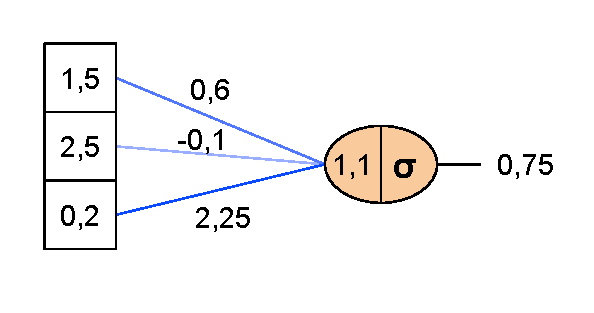
\includegraphics[width=\columnwidth]{figures/1neuron.pdf}%
\caption{Schéma d'un neurone avec trois connexions entrantes.}%
\label{fig:1neuron}%
\end{figure}

\subsection{Perceptron multi-couche}

Avec ce modèle simple de neurones, on peut définir un ensemble de neurones connectés les uns aux autres.
Un réseau de neurones profond entièrement connecté à plusieurs couches, appelé Perceptron multicouche, est un ensemble de neurones connectés, organisés en couches successives. 
Sur la figure~\ref{fig:perceptron}, nous voyons une couche de neurone entièrement connectée (en anglais Fully Connected Layer), avec un vecteur en entrée de taille $4$ et une sortie de taille $3$.
Une telle configuration avec $i$ neurones, produisant la sortie $y$ de taille $i$ grâce à l'entrée $x$ de taille $n$, peut être calculé de la manière suivante :

\begin{equation}
	\forall y_i \in y, y_i = \sigma \left ( \sum_{j=0}^{n} (x_j*w_j + b_i) \right ) 
\label{eq:layer}
\end{equation}


\begin{figure}[!htb]
  \begin{subfigure}{0.49\textwidth}
		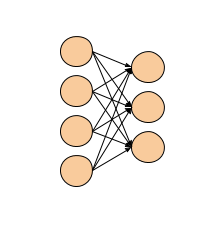
\includegraphics[width=\linewidth]{figures/Perceptron.png}
		\caption{Réseau à 1 couche} \label{fig:perceptron}
	\end{subfigure}
	\hspace*{\fill} % separation between the subfigures
	\begin{subfigure}{0.49\textwidth}
		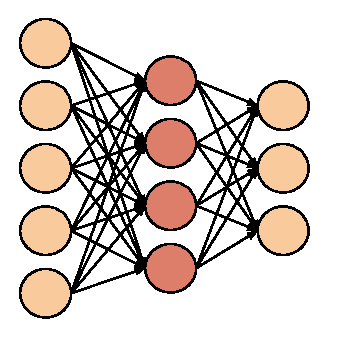
\includegraphics[width=\linewidth]{figures/MLP.pdf}
		\caption{Réseau à 2 couches} \label{fig:mlp}
	\end{subfigure}
	\caption{Réseaux de neurones à 1 et 2 couches.}
\end{figure}

Une couche ainsi définie est une classifieur linéaire, qui réalise sa prédiction grâce à une combinaisons des entrées.
Pour réaliser des fonctions plus complexes, des modèles avec une couche profonde sont nécessaires.
La figure~\ref{fig:mlp} représente un modèle avec deux couches entièrement connectées, avec ce que l'on nomme une couche cachée, en rouge sur le schéma.
Ces réseaux n'ont pas de connexions depuis la sortie vers l'entrée, ils sont nommés réseau à propagation avant (en anglais ``feed-forward networks''). 
À l'inverse les modèles avec des connexions allant de la sortie vers l'entrée sont appelés réseaux récurrents (cf section~\ref{sec:stateVideo}).
Chaque couche peut avoir une dimension arbitraire, et on remarque que le nombre de paramètres du réseau augmente rapidement.
Sur l'exemple de la figure~\ref{fig:mlp}, nous avons deux couches, la première ayant $5*4 + 4 =24$ paramètres et la deuxième $4*3 + 4 = 16$ en comptant les poids et les biais, ce qui fait $40$ paramètres à apprendre.

Le théorème d'approximation universelle~\cite{hornik1991approximation} stipule qu'un réseau de neurones avec une couche cachée peut approximer toute fonction continue sur un sous-ensemble compact de $\mathbb{R}^n$, à condition d'avoir une fonction d'activation continue, non-constante, bornée et croissante.
Ce qui fait d'un perceptron multi-couche un approximateur universel, du moins en théorie, rien ne garanti qu'il soit possible de trouver une telle fonction par apprentissage.







\subsection{Apprentissage des paramètres du réseau}

Pour que notre réseau profond réalise la fonction que l'on désire, il est nécessaire d'apprendre chacun de ses paramètres.
L'apprentissage se fait par mise à jour des poids $W$, par descente de gradient:

\begin{equation}
W = W - \alpha \frac{dL(\hat{y}, y)}{dW}
\label{eq:sgd}
\end{equation}

où $\alpha$ est la \textit{learning-rate}, qui définit de combien vont être ajusté les poids à chaque mise à jour. 
$L(\hat{y}, y)$ est la fonction objectif, ou fonction de coût, qui évalue si la sortie $y$ de notre réseau est correcte par rapport à la distribution attendue $\hat{y}$.
$\frac{dL(\hat{y}, y)}{dW}$ est la dérivée partielle de la fonction $L$, par rapport à chaque poids $W$, qui nous indique dans quel sens mettre à jour les poids (augmenter ou diminuer).


\begin{figure}%
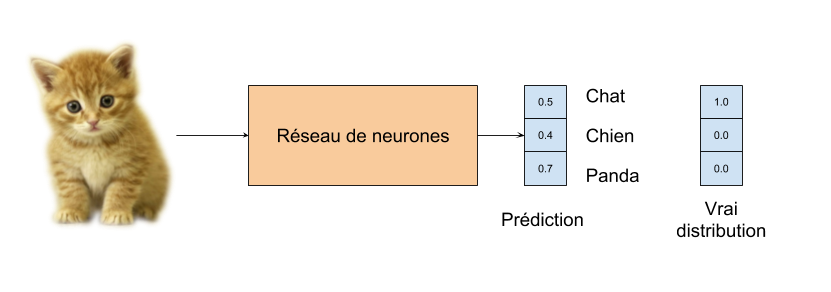
\includegraphics[width=\columnwidth]{figures/Apprentissage.png}%
\caption{Exemple d'apprentissage d'un réseau de neurone.}%
\label{fig:learning}%
\end{figure}

Prenons comme exemple la sortie d'un réseau de classification, présenté sur la figure~\ref{fig:learning}.
\'Etant donnée une image, le réseau de neurones va produire une sortie $q = (0.5, 0.4, 0.7)$. 
La distribution attendue $p = (1.0, 0.0, 0.0)$, correspond aux labels corrects de l'image.
On peut alors calculer l'entropie croisée, notée $CE$, grâce à l'équation~\ref{eq:sum4}, ce qui donne:

\begin{equation}
	CE(p,q) = -1*log(0.5) = 0,693 
\label{eq:crossapplied}
\end{equation}


Plus le réseau produit une distribution avec une grande confiance dans la bonne catégorie, plus l'entropie croisée sera proche de 0, et inversement.
Minimiser cette fonction par descente de gradient sur l'ensemble du réseau va permettre d'obtenir la bonne distribution en sortie du réseau, ce qui en fait une fonction objectif de choix.
On voit cependant que l'entropie croisée ainsi définie ne regarde que le score sur la bonne catégorie pour évaluer si la prédiction est correcte ou non.
Des approches récentes proposent ce qu'ils nomment ``label smoothing'' pour prendre un compte toutes les catégories, comme méthode de régularisation.
La régularisation dans les réseaux de neurones est très importante et permet de générer des modèles plus généraux, et d'éviter le sur-apprentissage (cf section~\ref{sec:regularisation}).

On parle de convergence si l'évolution de l'ensemble des paramètres est capable de trouver (de converger vers) des valeurs permettant de produire une réponse correcte en sortie du réseau.
Pour mettre à jour ces paramètres, on utilise la descente de gradient par lots.
Un lot (ou \textit{batch}) est un sous ensemble de l'ensemble des exemples $x$. 
C'est un moyen d'organiser les données d'apprentissages en paquets. 
Si l'on parcourt l'ensemble de ces lots de taille $S$, on parle alors d'une \textit{epoch}. 

\begin{equation}
W = W - \alpha \frac{1}{S} \sum_{j=1}^S \frac{dL(\hat{y}_j, y_j)}{dW}
\label{eq:sgdbatch}
\end{equation}

L'utilisation de \textit{batchs} permet d'accélérer l'apprentissage en profitant de la parallélisation, et peut réduire le bruit amené par l'utilisation de chaque exemple indépendamment.
On peut contrôler facilement la quantité de mémoire nécessaire pour l'apprentissage en jouant sur $S$, et le calcul du gradient peut être fait sur le \textit{batch} en entier, ce qui accélère grandement les calculs.
La stratégie classique consiste à mélanger aléatoirement les exemples pour chaque \textit{epoch}, et des les organiser en \textit{batch} de taille 16 à 64~\cite{bengio2012practical}.
Cependant, il a été démontré que l'utilisation de \textit{batchs} trop grands détériore les résultats et empêche d'avoir une bonne généralisation~\cite{masters2018revisiting}.












\begin{oframed}

%%%%%%%%%%%%%%%%%%%%%%      APARTE                %%%%%%%%%%%%%%%%%%%%%%%%%%%%%%%%%%%%%%%%%%%%%%%%%%%%%%%%%%%%%%
%\vspace{5mm}
%\begin{center}
%\begin{tcolorbox}[breakable, enhanced]
%\justify
\textbf{Cross-entropy : }
on utilise principalement l'entropie-croisée $CE$ comme fonction objectif, pour les raisons suivantes : 


Nous nous intéressons tout d'abord à l'entropie.
Prenons la loi de distribution de probabilité $p$ et un ensemble de $n$ exemples $(x_1, x_2, ..., x_n)$.
L'entropie de Shannon~\cite{shannon2001mathematical} nous indique le nombre de bits nécessaires pour la représentation de $p$, et est définie par :

\begin{equation}
E(p) = -\sum_{i=0}^n p(x_i) log p(x_i)
\label{eq:entropie}
\end{equation}

La dernière couche d'un réseau de neurones peut être un \textit{softmax}, c'est-à-dire avoir des valeurs comprises entre $0$ et $1$, avec une somme à $1$.
Dans ce cas, la sortie du réseau peut être vue comme une distribution $q$ qui doit estimer $p$, la vrai distribution.
Nous pouvons calculer la divergence de Kullback-Leibler qui nous donne la différence moyenne du nombre de bits nécessaires pour représenter $q$ par rapport à $p$.
La divergence de Kullback-Leibler entre $p$ et $q$ est définie par :

\begin{equation}
D_{KL}(p,q) = \sum_{i=0}^n p(x_i) log \frac{p(x_i)}{q(x_i)}
\label{eq:dkl}
\end{equation}

On veut minimiser la différence entre $q$ et $p$, ce qui revient à minimiser la somme de l'entropie de $p$ et de la divergence de Kullback-Leiber de $q$ par rapport à $p$. 

\begin{align}
 E(p) + D_{KL}(p,q) &= -\sum_{i=1}^n p(x_i) log p(x_i) + \sum_{i=0}^n p(x_i) log \frac{p(x_i)}{q(x_i)} \label{eq:sum1} \\
										&= \sum_{i=1}^n p(x_i) \left ( -log p(x_i) + log \frac{p(x_i)}{q(x_i)} \right ) \label{eq:sum2} \\
										&= \sum_{i=1}^n p(x_i) \left ( -log p(x_i) + log p(x_i) - log q(x_i) \right ) \label{eq:sum3} \\
										&= - \sum_{i=1}^n p(x_i) \left ( log q(x_i) \right ) = CE(p,q) \label{eq:sum4}
\end{align}
 
%\end{tcolorbox}
%\end{center}
%\vspace{5mm}

\end{oframed}

%%%%%%%%%%%%%%%%%%%%%%      FIN APARTE              %%%%%%%%%%%%%%%%%%%%%%%%%%%%%%%%%%%%%%%%%%%%%%%%%%%%%%%%%%%%%%


Chaque opération réalisée par le réseau étant dérivable, on va mettre à jour les poids par rétro-propagation du gradient, de la sortie vers l'entrée.
Ceci n'empêche pas que l'on risque de finir dans un minimum local, c'est-à-dire que la descente de gradient ne permettra plus l'amélioration des performances, alors qu'il existe un minimum global où le réseau serait meilleur.
Cependant, en pratique, il n'est pas constaté l'existence particulière de problème avec les minimum locaux, et la plupart des apprentissages donne des résultats similaires, avec des initialisations aléatoires du réseau au départ.
Il a d'abord été conjecturé qu'il n'existait pas de minimums locaux~\cite{lecun1989backpropagation}, mais il a été prouvé que tous les minimum locaux sont des minimums globaux pour les réseaux de quelques couches, bien que quelques minimum non-optimaux puissent exister dans les réseaux plus profonds~\cite{kawaguchi2016deep}.







%%%%%%%%%%%%%%%%%%%%%%%%%%%%%%%%%%%%%%%%%%%%%%%%%%%%%%%%%%%%%%%%%%%%%%%%%%%%%%%%%%%%%%%%%%%%%
\subsection{Non-linéarité et fonctions d'activation}

La fonction d'activation des neurones apporte la non-linéarité des connexions.
Les fonctions d'activation non linéaires peuvent être très variées et ont évoluées au fur et à mesure des années, mais on peut en relever trois principales.
Historiquement, la fonction sigmoïde fût la première proposée, elle est définie par:

\begin{equation}
	\sigma(x)= \frac{1}{1+\text{e}^{-x}}
\label{eq:sigmoid}
\end{equation}

Cette fonction projette les nombres réels dans $ \left [0,1 \right ]$, plus particulièrement les grands nombres deviennent $1$ et les plus petit nombres deviennent $0$ (figure~\ref{fig:sigmoid}).
La fonction sigmoïde est moins utilisée aujourd'hui car elle a tendance à réduire le gradient à zéro lors de la rétro-propagation.
Un autre désavantage de cette fonction est qu'elle n'est pas centrée sur $0$. 
Ce qui signifie que les couches suivantes dans le réseau recevront des données qui ne sont pas centrée sur $0$, ce qui est problématique pour le calcul du gradient.
Si on prend la dérivée partielle de $L$ en fonction de $w_i$:

\begin{equation}
	\frac{dL}{dw_i} = \frac{dL}{df} \frac{df}{dw_i}
	\label{eq:deriveN1}
\end{equation}

or d'après l'équation~\ref{eq:weightsum} :

\begin{equation}
	\frac{df}{dw_i} = x_i
	\label{eq:deriveN2}
\end{equation}

et donc 

\begin{equation}
	\frac{dL}{dw_i} = \frac{dL}{df}x_i
	\label{eq:deriveN3}
\end{equation}

Or si $x_i > 0$, le gradient $\frac{dL}{dw_i}$ sur les poids $w_i$ sera toujours du même signe (positif ou négatif) que $\frac{dL}{df}$.
Avec tous les gradients de même signe, tous les poids vont être mis à jour dans le même sens (augmentés ou diminués).
Ceci va créer un effet de ``zig-zag'' lors de la mise à jour des poids, avec une mise à jour dans un sens, puis dans un autre.

Ce problème n'apparait pas avec la fonction tangente hyperbolique (figure~\ref{fig:tanh}) :

\begin{equation}
tanh(x) = \frac{1-\text{e}^{-2x}}{1+\text{e}^{-2x}} = 2\sigma(2x) - 1
\label{eq:tanh}
\end{equation}

qui correspond en fait à la fonction sigmoïde centrée sur zéro, avec une sortie entre $ \left [-1,1 \right ]$.
Cette fonction est généralement à préférer à la fonction sigmoïd~\cite{lecun2012efficient}.

Cependant, la fonction ReLU pour Rectified Linear Unit~\cite{glorot2011deep}, est celle qui s'est le plus répandue ces dernières années et qui est largement la plus utilisée.
Elle est définie comme un seuil à zéro :

\begin{equation}
 ReLU(x) = max(0,x)
\label{eq:relu}
\end{equation}

La figure~\ref{fig:relu} présente graphiquement cette équation.
Cette fonction accélère grandement la convergence, ce qui serait dû à sa linéarité lorsque $f$ est positive, ce qui évite la saturation comme la tangente hyperbolique~\cite{krizhevsky2012imagenet}.
Un avantage considérable de cette fonction est sa facilité de calcul, qui ne requiert qu'un filtrage de la matrice d'activation avec un seuil à $0$.
Le fait de mettre un certain nombre de neurones à $0$ peut inactiver une partie du réseau qui au final ne sera jamais activé.
Pour éviter cette ``mort'' d'une partie du réseau, le Leaky ReLU a été proposé~\cite{he2015delving}, mais avec des résultats peu stables, il ne s'est pas généralisé.
Cette fonction, proche du ReLU, ajoute un paramètre $\alpha$ qui doit être appris, lorsque $x$ est négatif.

\begin{equation}
	f(n) =
  \begin{cases}
    \alpha x & \quad \text{if } x < 0 \\
    x  & \quad \text{if } x > 0
  \end{cases}
\label{eq:leakyrelu}
\end{equation}

\begin{figure}[!htb]
  \begin{subfigure}{0.49\textwidth}
		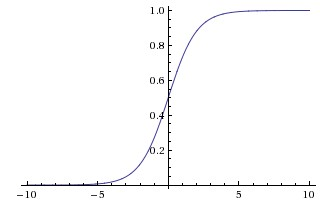
\includegraphics[width=\linewidth]{figures/sigmoid.jpeg}
		\caption{Sigmoïde} \label{fig:sigmoid}
	\end{subfigure}
	\hspace*{\fill} % separation between the subfigures
	\begin{subfigure}{0.49\textwidth}
		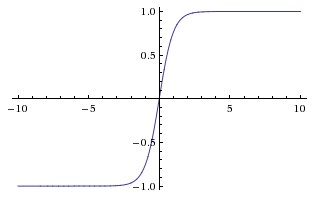
\includegraphics[width=\linewidth]{figures/tanh.jpeg}
		\caption{Tangeante Hyperbolique} \label{fig:tanh}
	\end{subfigure}
	\begin{subfigure}{0.49\textwidth}
		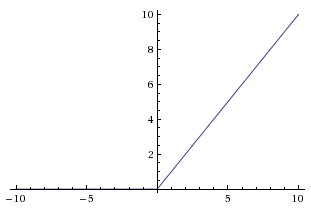
\includegraphics[width=\linewidth]{figures/relu.jpeg}
		\caption{ReLU} \label{fig:relu}
	\end{subfigure}
	\begin{subfigure}{0.49\textwidth}
		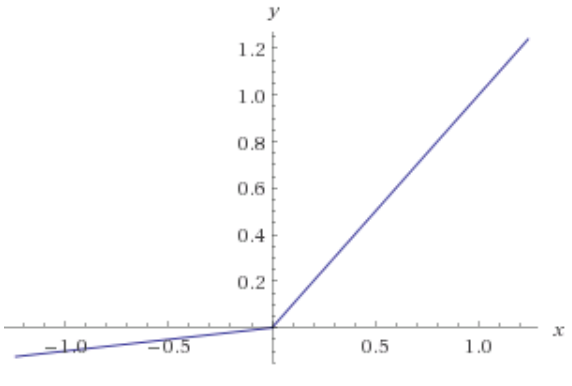
\includegraphics[width=\linewidth]{figures/lrelu.png}
		\caption{Leaky ReLU~\cite{he2015delving}} \label{fig:lrelu}
	\end{subfigure}
	\caption{Fonctions d'activation non-linéaires.}
	\label{fig:activation}
\end{figure}




\subsection{Régularisation}
\label{sec:regularisation}

Lorsque l'on réalise un algorithme d'apprentissage automatique, on souhaite que celui-ci n’ait pas uniquement de bonnes performances sur les données d'apprentissages, mais sur toutes données qu'on lui présente.
La régularisation est l'ensemble des méthodes qui permettent à l'algorithme de réduire son erreur de généralisation.

\vspace{5mm}
\begin{center}
	\fbox{
\begin{minipage}{.99\textwidth}
\justify
\textbf{Généralisation} : capacité d'un réseau de neurones, et de n'importe quel algorithme d'apprentissage automatique, à bien se comporter sur des données qu'il n'a pas vu pendant l'entrainement. Généralement mesuré grâce à un corpus de test séparer du corpus d'entraînement. Un exemple extrême d'un algorithme qui généralise mal, est un réseau capable d'atteindre 100\% de reconnaissance sur les données fournies pendant l'apprentissage et 0\% sur le corpus de test. On parle de \textbf{sur-apprentissage}~\cite{srivastava2014dropout}.
\end{minipage}
}
\end{center}
\vspace{5mm}


Une façon schématique de voir la régularisation est d'imaginer un ajout de bruit dans les réseaux pour les rendre plus robustes et moins spécialisés sur leurs données d'apprentissages.
L'idée est donc de déstabiliser le réseau lors de l'apprentissage, pour qu'il ne soit pas limité aux exemples fournis pendant l'apprentissage, dans le but d'éviter un sur-apprentissage.

\vspace{5mm}
\begin{center}
	\fbox{
\begin{minipage}{.99\textwidth}
\justify
\textbf{Sur-apprentissage} : On parle de sur-apprentissage lorsqu'un réseau de neurones s'est trop spécialisé sur ses données d'apprentissages et qu'il a une forte erreur de généralisation.
\end{minipage}
}
\end{center}
\vspace{5mm}

L'augmentation de données consiste à perturber les images pendant l'apprentissage, avec du bruit, des rotations ou des mises à l'échelle.
On peut citer par exemple le \textit{crop} aléatoire, où l'on prend aléatoirement une zone de l'image plutôt que de mettre l'image à l'échelle pour l'entrée du réseau.
On utilise également fréquemment des rotations des images, avec des renversement aléatoire de l'image, entre $ \left [ -180^\circ, 180^\circ \right ] $.
Il est également possible de modifier les contrastes, la teinte ou la saturation, toujours dans le but de déformer les images pour montrer le plus d'exemples différents possible au réseau.

Une forme de régularisation importante et utiliser dans tous les apprentissages aujourd'hui est le ``weight decay'', ou la normalisation L2 des poids.
Les poids sur les connexions de chaque neurones peuvent prendre des valeurs de forte amplitude pendant l'apprentissage, or cela est pénalisant pour la généralisation, en créant une variance de sortie plus élevée~\cite{hanson1989comparing, krogh1992simple}.
On souhaite donc forcer les poids à rester petits en pénalisant les grandes valeurs.
En utilisant la norme L2 avec un paramètre $\alpha$:

\begin{equation}
	W = \alpha \sum_{i=1}^n w_i
\label{eq:weightDecay}
\end{equation}

On force ainsi les poids à rester dans une sphère de rayon $\alpha$.
Ce paramètre est un ~\textit{hyper-paramètre} à optimiser pendant l'apprentissage, et va dépendre de chaque réseau, avec des valeurs généralement faibles entre $10^{-3}$ et $10^{-4}$.


Une autre forme de régularisation largement utilisée est le ~\textit{dropout}~\cite{srivastava2014dropout}.
Il s'agit de masquer une partie du réseau aléatoirement pendant l'apprentissage.
Pour cela, chaque neurone du réseau a une probabilité $p$ d'être abandonné (dropped) à chaque passage.
La figure~\ref{fig:dropout} montre à gauche le réseau initial, et à droite un exemple avec $7$ neurones abandonnés, noté X.
Une fois l'apprentissage terminé avec ces coupes aléatoires, toutes les connexions sont utilisées lorsque l'on déploie le réseau.
Ceci entraîne une activation totale supérieure, car aucune connexion n'est ignorée. 
Pour garder une activation du même ordre de grandeur que pendant l'entrainement, elles sont toutes réduites d'un facteur $p$.

\begin{figure}%
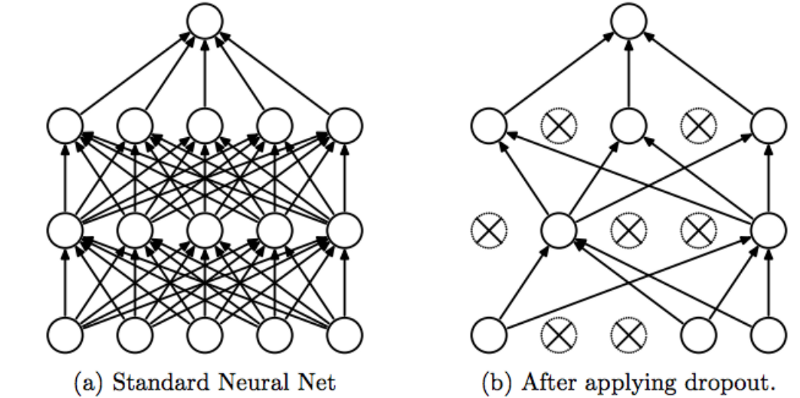
\includegraphics[width=\columnwidth]{figures/dropout.png}%
\caption{Illustation du ~\textit{dropout} pris depuis ~\cite{srivastava2014dropout}}%
\label{fig:dropout}%
\end{figure}


Les régularisations que nous venons de présenter ne se font qu'au niveau d'un exemple.
Il est toutefois possible d'agir directement au niveau du ~\textit{batch}, lot de données utilisé pendant l'apprentissage.
La normalisation du \textit{batch} (\textit{batch-normalisation}), n'est pas prévue à l'origine pour faire de la régularisation~\cite{ioffe2015batch}.
Utiliser dans les modèles performants récent~\cite{szegedy2016rethinking, he2016deep, hu2017squeeze}, cette méthode n'est pas dédiée à la régularisation, mais améliore effectivement les capacités de généralisation. 

\vspace{5mm}
\begin{center}
\fbox{
\begin{minipage}{.99\textwidth}
\justify
\textbf{NORMALISATION} : on désigne par normalisation le fait de centrer-réduire les données (soustraire la moyenne et diviser par l'écart-type). On préfère le terme normalisation ici pour être cohérent l'appellation largement répandue: \textit{batch-normalisation}.
\end{minipage}
}
\end{center}
\vspace{5mm}


Cette \textit{batch normalisation} est utilisée pour accélérer l'apprentissage, en forçant toutes les données à être centrées sur 0.
En apprentissage automatique, on centre et réduit généralement les données pour éviter d'avoir à apprendre un décalage en plus de la représentation.
L'idée de la normalisation du ~\textit{batch} est de faire cette opération entre chaque couche, pour que les données soient toujours centrées et réduites.
Ceci a deux principales conséquences : on peut utiliser un \textit{learning rate} plus grand car on évite les activations trop grandes ou trop petites, et on limite le sur-apprentissage en ajoutant du bruit entre chaque couche car la variance va dépendre du \textit{batch}.
Pour le déploiement du réseau après l'entraînement, la moyenne et l'écart-type utilisés pour la normalisation ne dépendent plus du \textit{batch}, on prend ceux de la population (calculé sur l'ensemble des données d'apprentissage).

On voit sur le tableau~\ref{tab:regularization} les effets de chacune des régularisations sur deux réseaux profonds classiques, AlexNet et Inception (cf section~\ref{sec:cnn}) sur la collection d'image ImageNet~\cite{deng2009imagenet}.
On y présente l'effet de l'augmentation de données (Aug. D), du \textit{weight decay} (W.D.) et de la normalisation du \textit{batch} (BatchNorm).
Les résultats montrent que, malgré les perturbations apportées par les différentes fonctions, les réseaux parviennent toujours à obtenir des résultats proches de 100\% sur le corpus d'apprentissage, en particulier Inception, qui est le réseau le plus performant sur cette tâche.
Ceci permet par contre d'améliorer significativement les résultats sur les corpus de test, avec une amélioration de plus de 7\% pour Inception et de plus de 5\% pour AlexNet.
On remarque avec Inception l’apport important de la normalisation du batch, avec de 3.76\% à elle seule.
On en conclut donc que ces fonctions de régularisations permettent d'améliorer la généralisations des réseaux sur des exemples qu'ils n'ont jamais vu\footnote{Cette affirmation est toutefois à prendre avec précaution, car étant donné la taille des réseaux, il est également possible qu'ils ne fassent que retenir toutes l'informations qu'on leur donne~\cite{zhang2016understanding}.}.


\begin{table}%
\centering
\begin{tabular}{|l||c|c|c||c|c|}
\hline
Modèle & Aug.D & W.D. & BatchNorm & P. entrainement & P. test \\
\hline
AlexNet & non & non & NA & 100 & 76.07 \\
AlexNet & non & oui & NA & 100 & 77.36 \\
AlexNet & oui & non & NA & 99.82 & 79.66 \\
AlexNet & oui & oui & NA & 99.90 & 81.22 \\
\hline
Inception v3 & non & non & non & 100 & 82.00 \\
Inception v3 & non & oui & non & 100 & 83.00 \\
Inception v3 & non & non & oui & 100 & 85.76 \\
Inception v3 & non & oui & oui & 100 & 86.03 \\
Inception v3 & oui & non & oui & 100 & 89.31 \\
Inception v3 & oui & oui & oui & 100 & 89.05 \\
\hline
\end{tabular}
\caption{Effets sur AlexNet et Inception de la régularisation~\cite{zhang2016understanding}}
\label{tab:regularization}
\end{table}







%%%%%%%%%%%%%%%%%%%%%%%%%%%%%%%%%%%%%%%%%%%%%%%%%%%%%%%%%%%%%%%%%%%%%%%%%%%%%%%%%%%%%%%%%%%%%
%																																														%
%																																														%
%																				Convolutions																				%
%																																														%
%																																														%
%%%%%%%%%%%%%%%%%%%%%%%%%%%%%%%%%%%%%%%%%%%%%%%%%%%%%%%%%%%%%%%%%%%%%%%%%%%%%%%%%%%%%%%%%%%%%
\section{Réseaux de neurones convolutifs}

Nous avons présenté les réseaux de neurones de type perceptrons multi-couches.
Notamment en traitement d'image, l’utilisation de convolutions, très répandues, permettent d'obtenir les meilleurs résultats de l'état de l'art~\cite{krizhevsky2012imagenet, simonyan2014very, he2016deep, hu2017squeeze}.


\subsection{Convolutions}


Une convolution est une opération entre une matrice $M$ et une matrice de convolution $K$, appelée \textbf{noyau}.
L'opération de convolution est définie comme la somme des éléments de $M$ pondérés par les éléments de $K$.
Si $K$ est une matrice carrée de dimension $2n+1$, alors on peut définir la matrice $G$ résultat de la convolution entre $M$ et $K$ par :

\begin{equation}
G[i,j] = \sum_{u=-n}^{n} \sum_{v=-n}^{n} K[u,v]*M[i-u, j-v]
\label{eq:conv}
\end{equation}

On peut visualiser cette opération sur la figure~\ref{fig:conv1}, où une matrice de convolution $K$ de taille $3*3$ est appliquée sur une matrice $M$ de taille $5*5$.
On obtient une matrice $G$ dont la taille va dépendre de la manière dont on applique le noyau sur $M$.
On voit dans l'équation~\ref{eq:conv}, que l'on considère que $M$ est toujours définie dans le voisinage de $[i,j]$, ce qui n'est bien entendu pas le cas en pratique, et génère des dépassement de matrice.

%\begin{figure}%
%\centering
%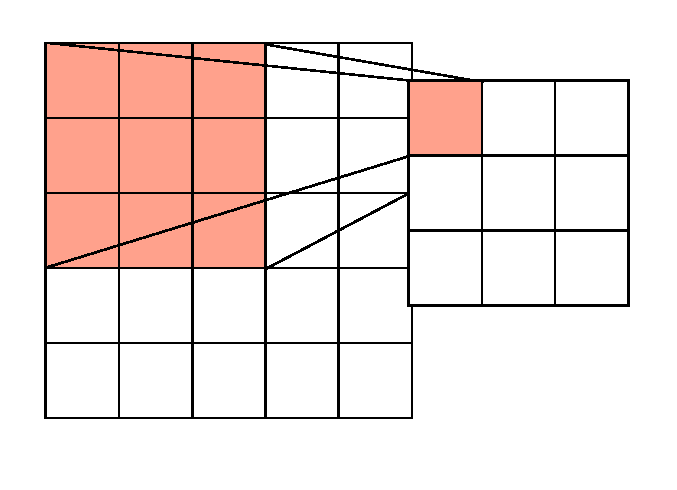
\includegraphics[width=.6\columnwidth]{figures/convolutionSimple.pdf}%
%\caption{Schéma de l'opération de convolution}%
%\label{fig:convS}%
%\end{figure}


On cherche donc à appliquer une matrice de convolution de taille $2n+1$ sur une matrice (on ne s'intéresse qu'aux convolution de taille impaire).
Pour cela on peut définir un pas de décalage entre chaque application.
Avoir un pas de 1 signifie que la convolution sera décalée d'un élément après chaque application, et donc qu'elle sera appliquée en chaque position possible de l'image.

\begin{figure}%
\centering
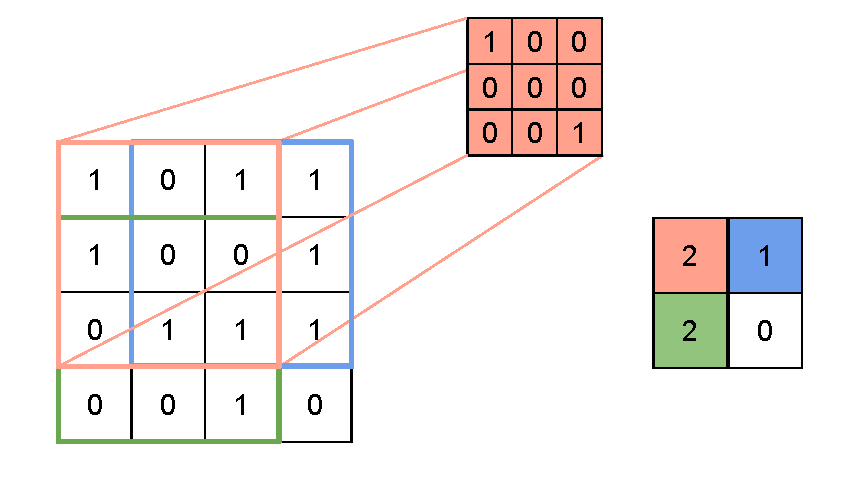
\includegraphics[width=.6\columnwidth]{figures/convolution.pdf}%
\caption{Illustration d'une convolution sur une matrice $4*4$.}%
\label{fig:conv1}%
\end{figure}

On peut ainsi calculer la taille de la sortie de la convolution d'une matrice carrée de taille $m$ par une matrice de convolution de taille $2*n+1 < m$ : $\frac{m-(2*n+1)}{s} + 1$.
Elle sera toujours inférieur à $m$, et donc la convolution va réduire la taille de la matrice d'entrée.
Cela vient du fait que la matrice de convolution ne peut pas être appliquée avec pour centre la première ou la dernière ligne ou colonne.
Pour corriger ce problème, on peut définir un remplissage (\textit{padding}) autour de la matrice $M$.
En ajoutant ligne et colonne de 0 autour de la matrice $M$ on va pouvoir appliquer la convolution sur un domaine plus grand, sans que cela ne perturbe le résultat, car en ajouter des 0 est sans effet dans l'équation~\ref{eq:conv}.
Comme on ajoute le padding de chaque côté de la matrice, la taille de la sortie sera : $\frac{m-(2n+1)+2p}{s} + 1$.
En prenant un padding de taille $p=n$, avec un pas de 1, on assure que la taille de la sortie sera égale à la taille de l'entrée (figure~\ref{fig:convpad}).

\begin{figure}%
\centering
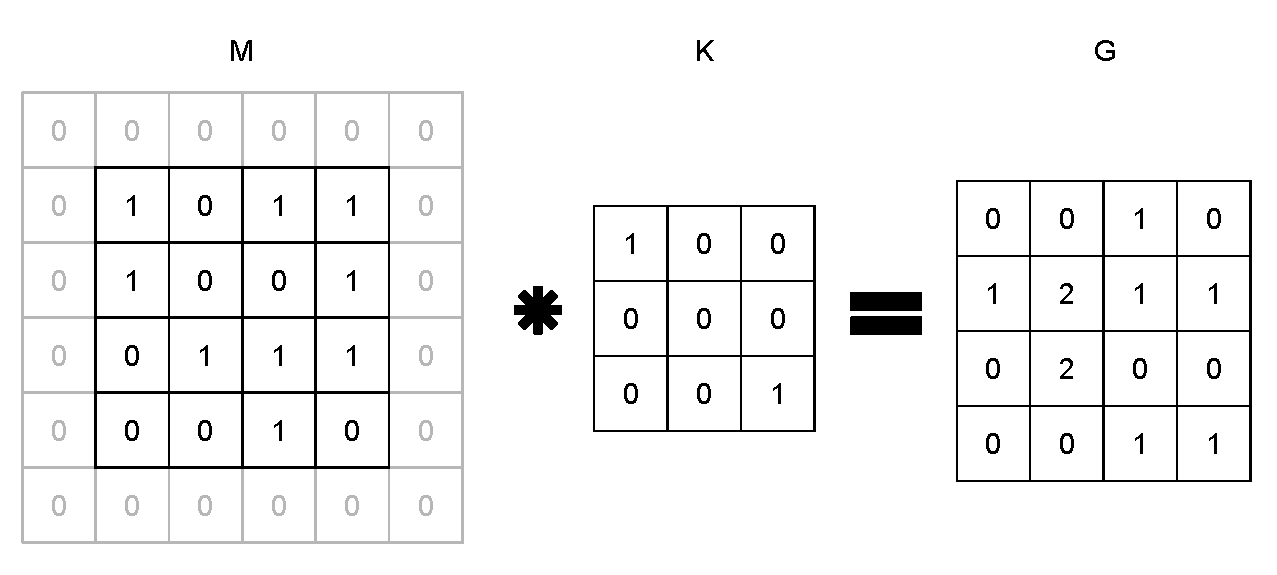
\includegraphics[width=\columnwidth]{figures/convolutionpadding.pdf}%
\caption{Application d'une convolution 3x3 sur une matrice de taille 4x4 avec un padding de 1 et un pas de 1}%
\label{fig:convpad}%
\end{figure}

Chaque couche d'un réseau convolutif profond va être définie par un ensemble de convolutions, dont la sortie peut être connectée à un neurone.
Une image n'étant pas une matrice en deux dimensions, mais un ensemble de matrices, on peut voir celle-ci comme une matrice 3D de taille $L*H*C$ où $L$ et $H$ sont la largeur et la hauteur de l'image, et $C$ le nombre de canaux.
Si on applique un certain nombre $K$ de convolutions sur celle-ci, on obtient une matrice 3D de taille $L*H*K$, si la taille d'entrée et de sortie sont identique, ce qui est illustré par la figure~\ref{fig:convMultiple}. 
En ensemble de convolutions comme celui-ci va définir une \textbf{couche de convolution}, composant de base pour un réseau convolutif.


\begin{figure}%
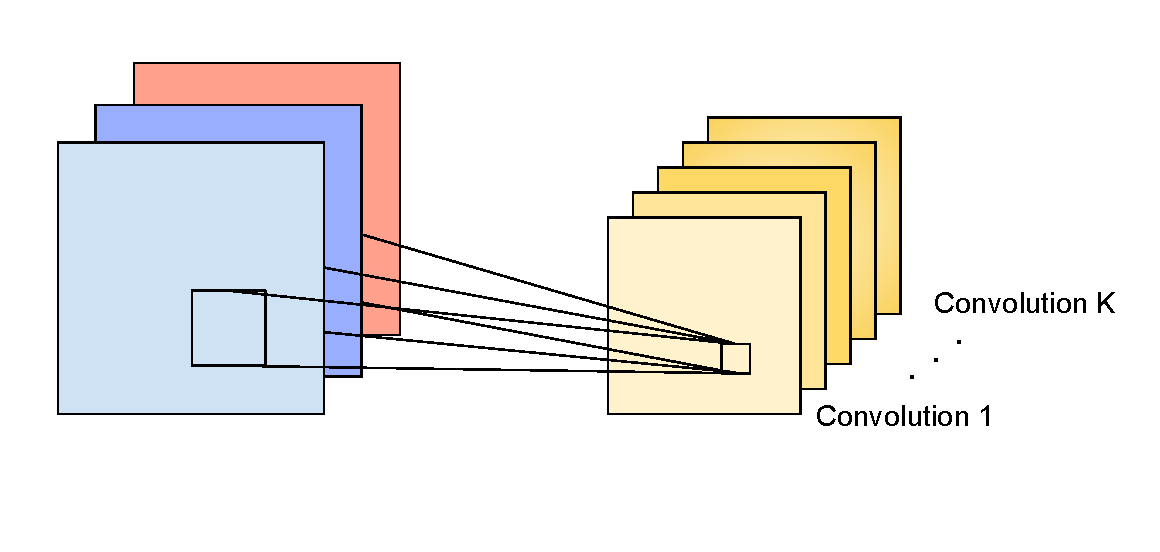
\includegraphics[width=\columnwidth]{figures/ConvolutionMultiple.pdf}%
\caption{Couche de convolution avec 3 canaux en entrée et 5 en sortie.}%
\label{fig:convMultiple}%
\end{figure}

D'autres opérations vont être appliquées pour définir un réseau convolutif, notamment des neurones, généralement de type ReLU, et du \textit{pooling}.
L'opération de pooling consiste à mettre en commun (\textit{to pool}) un certain nombre d'élément de la matrice. 
On prend généralement le maximum (max-pooling) ou la moyenne (average-pooling) d'une région, ce qui permet de faire un sous-échantillonnage, et donc une réduction de la taille de la matrice.
En appliquant une pooling $2*2$ avec un pas de 2 sur notre matrice $L*H*C$, on obtient la matrice $L/2 * H/2 * C$.
La figure~\ref{fig:operationlayer} montre les trois étapes d'une couche d'un réseau convolutif, avec une convolution (fig.~\ref{fig:catconv}), des neurones ReLU (fig.~\ref{fig:catrelu}) et du pooling (fig.~\ref{fig:catpool}).

\begin{figure}[htbp]
\centering
\begin{subfigure}{0.24\textwidth}
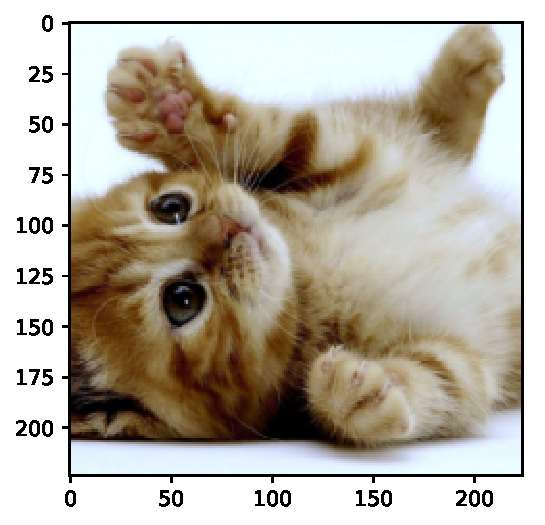
\includegraphics[width=\linewidth]{figures/cat.pdf}
\caption{Image d'origine} \label{fig:chaton}
\end{subfigure}
\hspace*{\fill} % separation between the subfigures
\begin{subfigure}{0.24\textwidth}
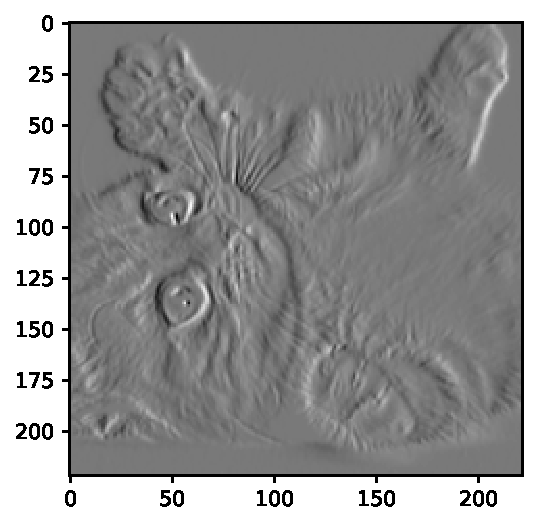
\includegraphics[width=\linewidth]{figures/catConv.pdf}
\caption{Convolution} \label{fig:catconv}
\end{subfigure}
\begin{subfigure}{0.24\textwidth}
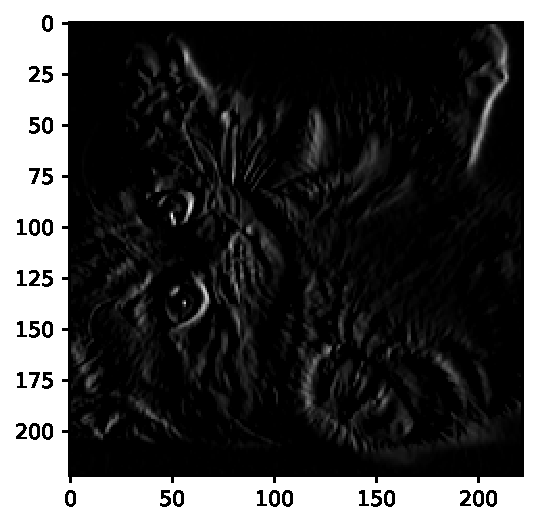
\includegraphics[width=\columnwidth]{figures/catRelu.pdf}
\caption{ReLU} \label{fig:catrelu}
\end{subfigure}
\hspace*{\fill}
\begin{subfigure}{0.24\textwidth}
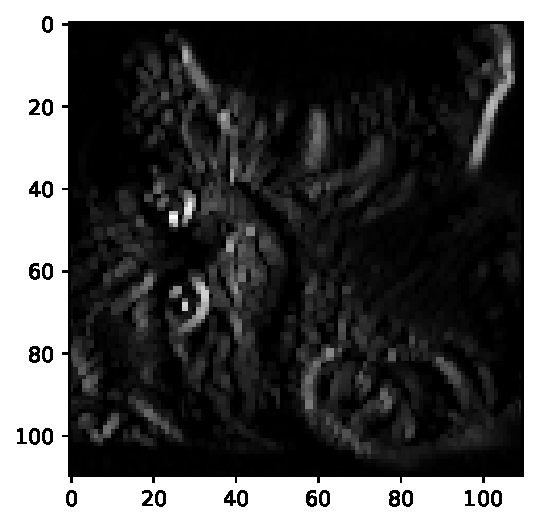
\includegraphics[width=\columnwidth]{figures/catPool.pdf}
\caption{Average Pooling} \label{fig:catpool}
\end{subfigure}


\caption{Illustration des opérations de convolution, de ReLU et de \textit{pooling}}
\label{fig:operationlayer}
\end{figure}



%\begin{figure}[ht!]
%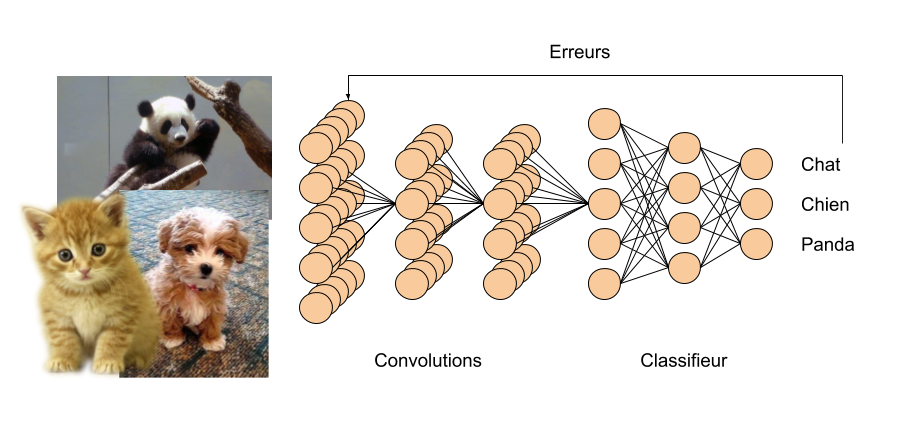
\includegraphics[width=\columnwidth]{figures/TrainDeepLearning.png}%
%\caption{Exemple d'apprentissage de classification à l'aide d'une réseau de neurones profond. Les poids sont mis à jour grâce à la rétro-propagation de l'erreur.}%
%\label{fig:dlclassification}%
%\end{figure}



\subsection{Réseaux convolutifs profonds}
\label{sec:cnn}

Nous nous intéressons à plusieurs réseaux convolutifs de l'état de l'art qui présentent les éléments les plus importants de tous les réseaux de neurones.
L'un des premiers réseaux de neurones convolutifs, et le premier à se répandre, est LeNet présenté par Lecun et al.~\cite{lecun1998gradient}, illustré par la figure~\ref{fig:lenet}. Ce réseau est constitué de deux couches de convolutions séparées par une couche de sous-échantillonnage (similaire à l'\textit{average-pooling}). 
Une partie entièrement connectée permet de passer d'une sortie de taille $16*5*5$ à une sortie de dimension 10, correspondant aux dix classes MNIST~\cite{lecun1998gradient}, la tâche de reconnaissance de chiffre pour laquelle le réseau a été développé.

\begin{figure}%
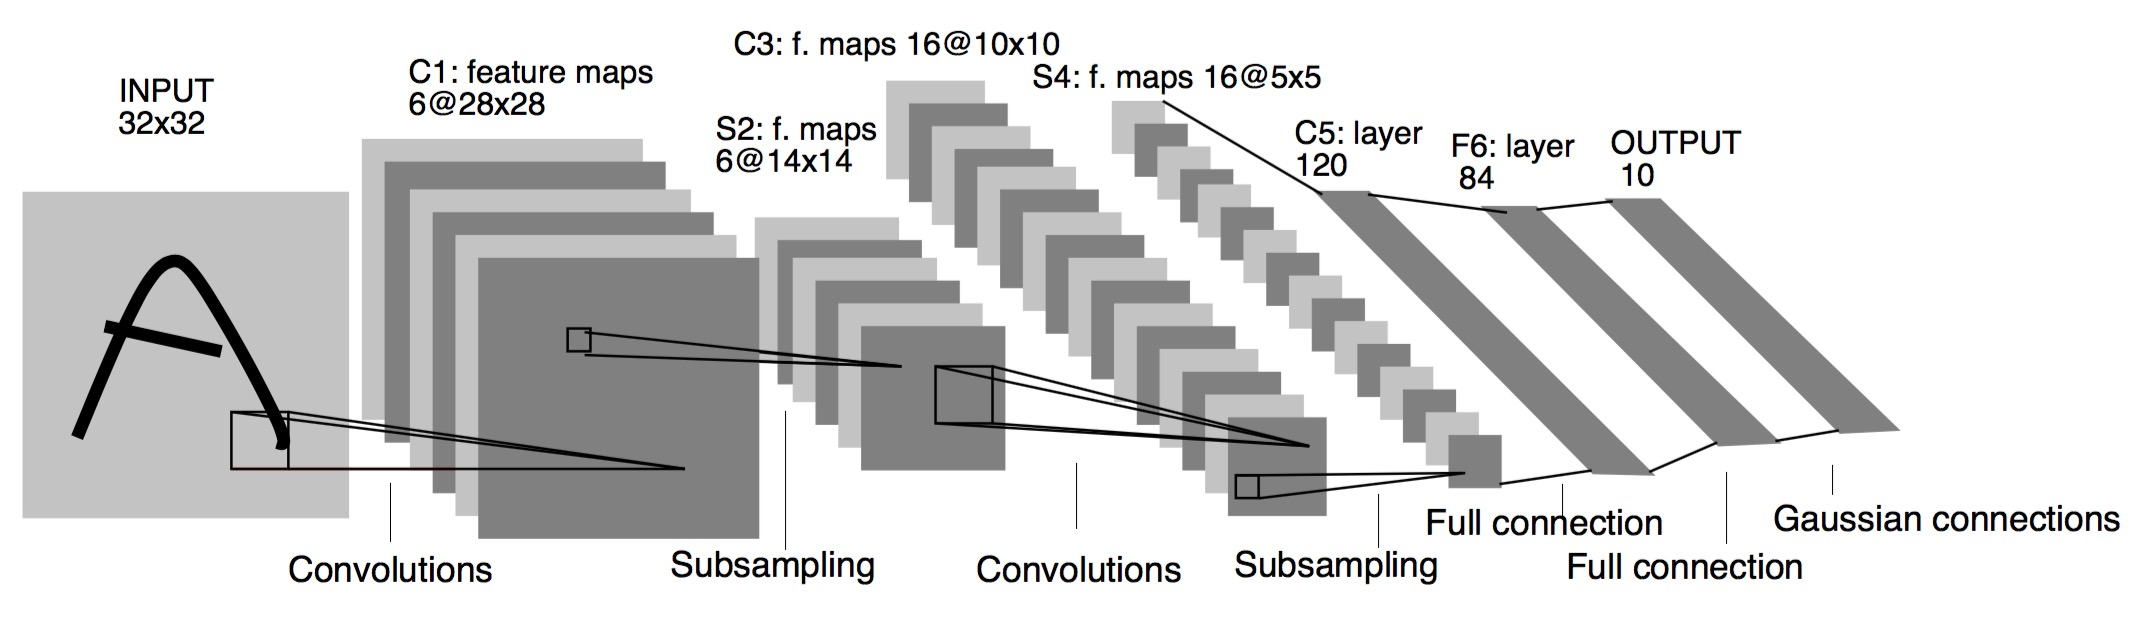
\includegraphics[width=\columnwidth]{figures/lenet5.jpg}%
\caption{Schéma du réseau profond LeNet~\cite{lecun1998gradient}}%
\label{fig:lenet}%
\end{figure}

Ce réseau dispose de toutes les briques nécessaires pour la construction de tous les réseaux convolutifs qui suivront.
Notamment avec une partie ``caractéristiques'', à savoir un ensemble de convolutions, qui sont chargées d'extraire les caractéristiques visuelles.
Et une partie ``classification'', avec des couches entièrement connectées, chargées de réaliser la classification en 10 catégories dans le cas présent.

%AlexNet -> dropout 
L'architecture AlexNet, présentée en 2012~\cite{krizhevsky2012imagenet} pour la tâche de classification ImageNet~\cite{deng2009imagenet}\footnote{La collection d'image ImageNet est très utilisée pour l'apprentissage des réseaux de neurones, car elle dispose de plusieurs millions d'images annotées, et répartit en plusieurs milliers de classes.}, utilise une approche similaire.
Bien que cette architecture soit largement plus grande, avec plus 60 millions de paramètres, l'organisation est proche de celle de LeNet (figure~\ref{fig:alexnet}), avec une partie extraction de caractéristiques, composée de cinq convolutions, et une partie classification composée de couches entièrement connectées.

\begin{figure}%
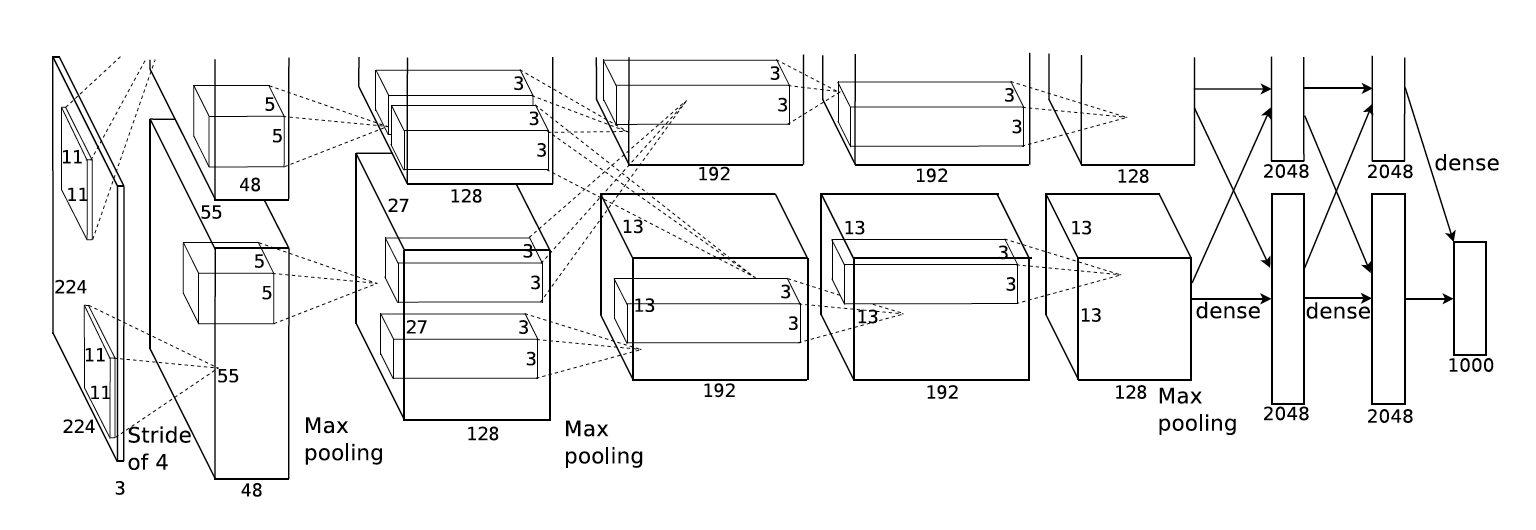
\includegraphics[width=\columnwidth]{figures/alexnet.png}%
\caption{Architecture AlexNet~\cite{krizhevsky2012imagenet}}%
\label{fig:alexnet}%
\end{figure}

Ce réseau utilise des convolutions de $11*11$ et de $3*3$, chacune séparée par un max-pooling de taille $3*3$, ce qui représente un grand nombre de sous-échantillonnage. 
Une des nouveautés de ce réseau est l'introduction des dropout (présentés section~\ref{sec:regularisation}), qui lui permettent de ne pas sur-apprendre, malgré sa grande taille.
Cette nouvelle architecture atteint 18.2\% d'erreur ImageNet\footnote{Ces résultats, et tout ceux qui suivent, sont basés sur une réimplémentation des réseaux, et peuvent différencier de ceux des publications originales. Nous nous intéressons surtout à l'ordre de grandeur et aux écarts entre les résultats, qui eux ne changent pas.}, ce qui est bien inférieur aux résultats précédent sans réseaux de neurones, qui étaient de 26.2\% avec les descripteurs visuels SIFT (Scale-Invariant Feature Transform)~\cite{sanchez2011high}.

Ces résultats sur un problème de vision bien connu ont permis au réseaux de neurones d'être à nouveau au centre de l'attention de la communauté scientifique.
Les nouveautés proposées par Simonyan et Zisserman~\cite{simonyan2014very} avec leur réseau VGG, ont posé de nouvelles bases pour la constructions de réseaux profonds.
Premièrement, ils proposent de n'utiliser que des convolutions $3*3$.
En utilisant des convolutions de petites tailles, on peut augmenter la profondeur du réseau, ce qui en pratique donne de meilleurs résultats.
Le réseau VGG présenté (figure~\ref{fig:vgg}) est plus profond, il utilise ici 16 couches, dont 13 de convolutions et 3 entièrement connectés pour la classification.
Une version avec 19 couches est également proposée.
Ceci fait passer le nombre de paramètres à 144 millions, et on commence alors à parler de réseaux \textit{très} profonds. 


\begin{figure}%
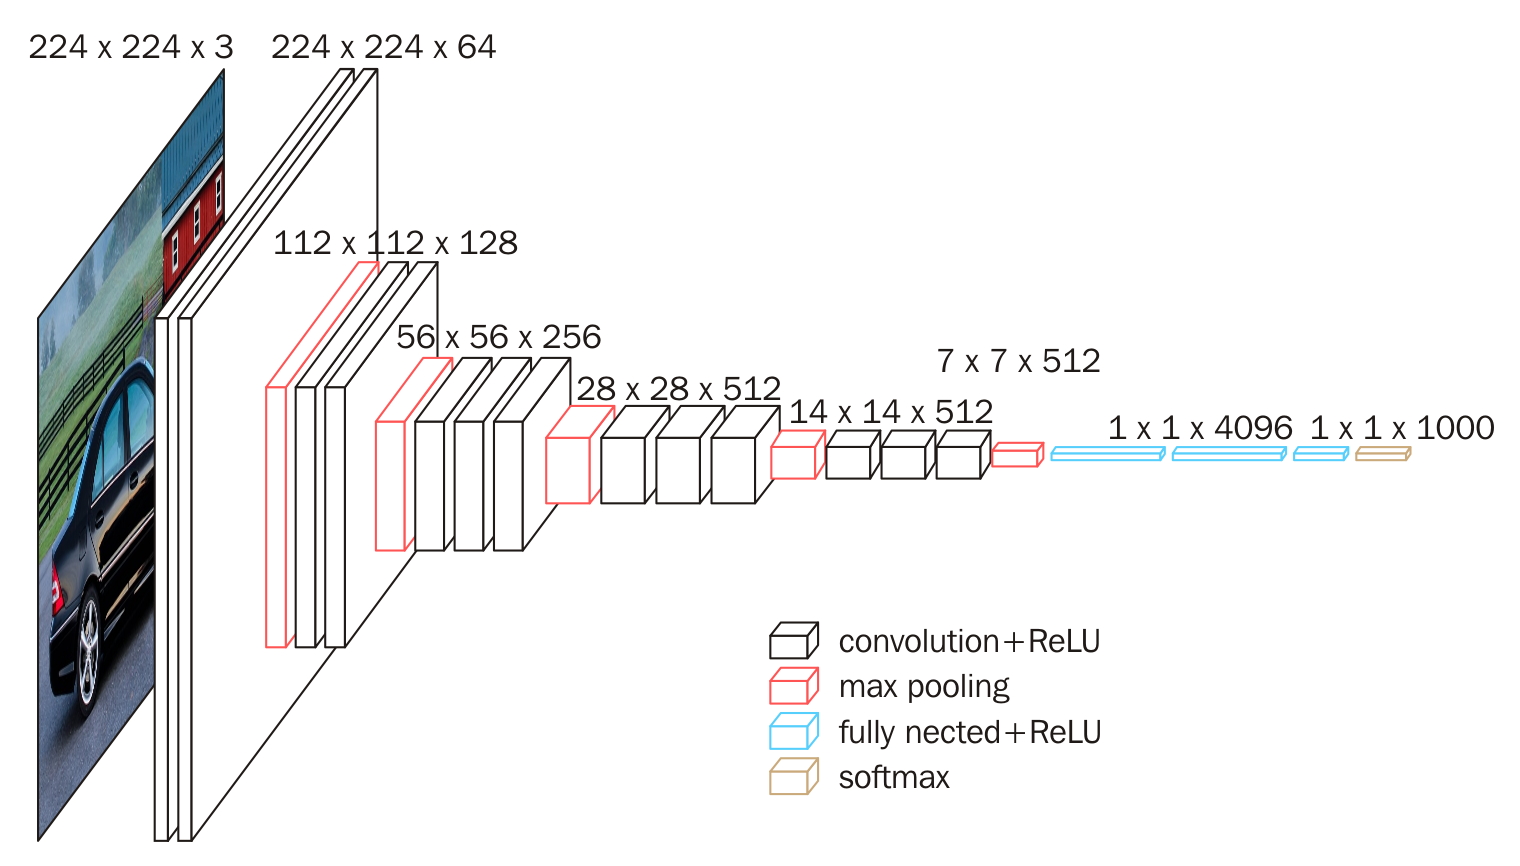
\includegraphics[width=\columnwidth]{figures/vgg.png}%
\caption{Architecture VGG~\cite{simonyan2014very}}%
\label{fig:vgg}%
\end{figure}
%VGG -> Uniform design : 3x3 uniquement, et downsampling with pooling. And when downsampling doubling the nb of channel.

Les convolutions $3*3$ ne sont pas toutes séparées par du sous-échantillonnage comme dans les réseaux précédent.
En effet, deux convolution $3*3$ à la suite ont le même champ récepteur qu'une convolution $5*5$, s'il n'y a pas de pooling entre les deux, et 3 à la suite ont le même qu'une convolution $7*7$.
Remplacer une convolution $7*7$ par trois convolution $3*3$ permet de multiplier par trois le nombre d'activations non-linéaires ReLU, ce qui rend la fonction plus discriminante, en plus de réduire considérablement le nombre de paramètres (81\% de paramètres en moins).
On obtient alors un réseau plus profond, et plus performant, arrivant à un taux d'erreur de 8.1\% sur ImageNet~\cite{simonyan2014very}.

En plus de se limiter à des convolutions $3*3$, VGG propose d'utiliser deux types de couches dans le réseau.
Premièrement des couches qui conserve la taille des entrées, donc avec un pas de 1 et un ~\textit{padding} de 1, et des couches qui réduise la taille par deux, avec un pas de 2, mais qui multiplient par deux le nombre de canaux.
En enchaînant ces deux types de couches, on peut construire un réseau de plus en plus profond, avec moins de disparition du gradient.
 

%ResNet -> skip-connection
Le problème de l'approfondissement des réseaux est la diminution du gradient au fur et à mesure de la rétro-propagation.
En effet, à chaque couche, le gradient va diminuer légèrement. 
Alors que ce n'est pas un problème pour des réseaux avec quelques couches, si l'on veut continuer à approfondir les réseaux, il réduire l'impact de cette diminution.
L'architecture de réseau ResNet~\cite{he2015delving} propose un nouveau type de connexion : les ~\textit{skip-connections}, ou plus précisément les connexions résiduelles.
Pour éviter que chaque couche fasse disparaître petit à petit le gradient, on ajoute une connexion de l'entrée de la convolution directement vers la sortie. 
Cela crée deux ``chemins'' pour la propagation et surtout la rétro-propagation.
Un exemple est montré sur la figure~\ref{fig:resnet}, avec un bloc résiduel, constitué de deux couches de convolutions et d'une connexion résiduelle entre l'entrée et la sortie.
Ici la fusion est faite avec une addition, ce qui montre les meilleurs résultats en pratique, car permet une meilleure propagation de l'information~\cite{he2016identity}.

\begin{oframed}

\textbf{Bloc :} avec la taille grandissante des réseaux de neurones, le terme blocs de convolutions a été introduit. Un bloc est un ensemble d'un certain nombre de couches d'un réseau. Cela permet de définir plus simplement des réseaux très profonds, quand certaines structures se répètent dans le réseau. 

\end{oframed}



\begin{figure}%
\centering
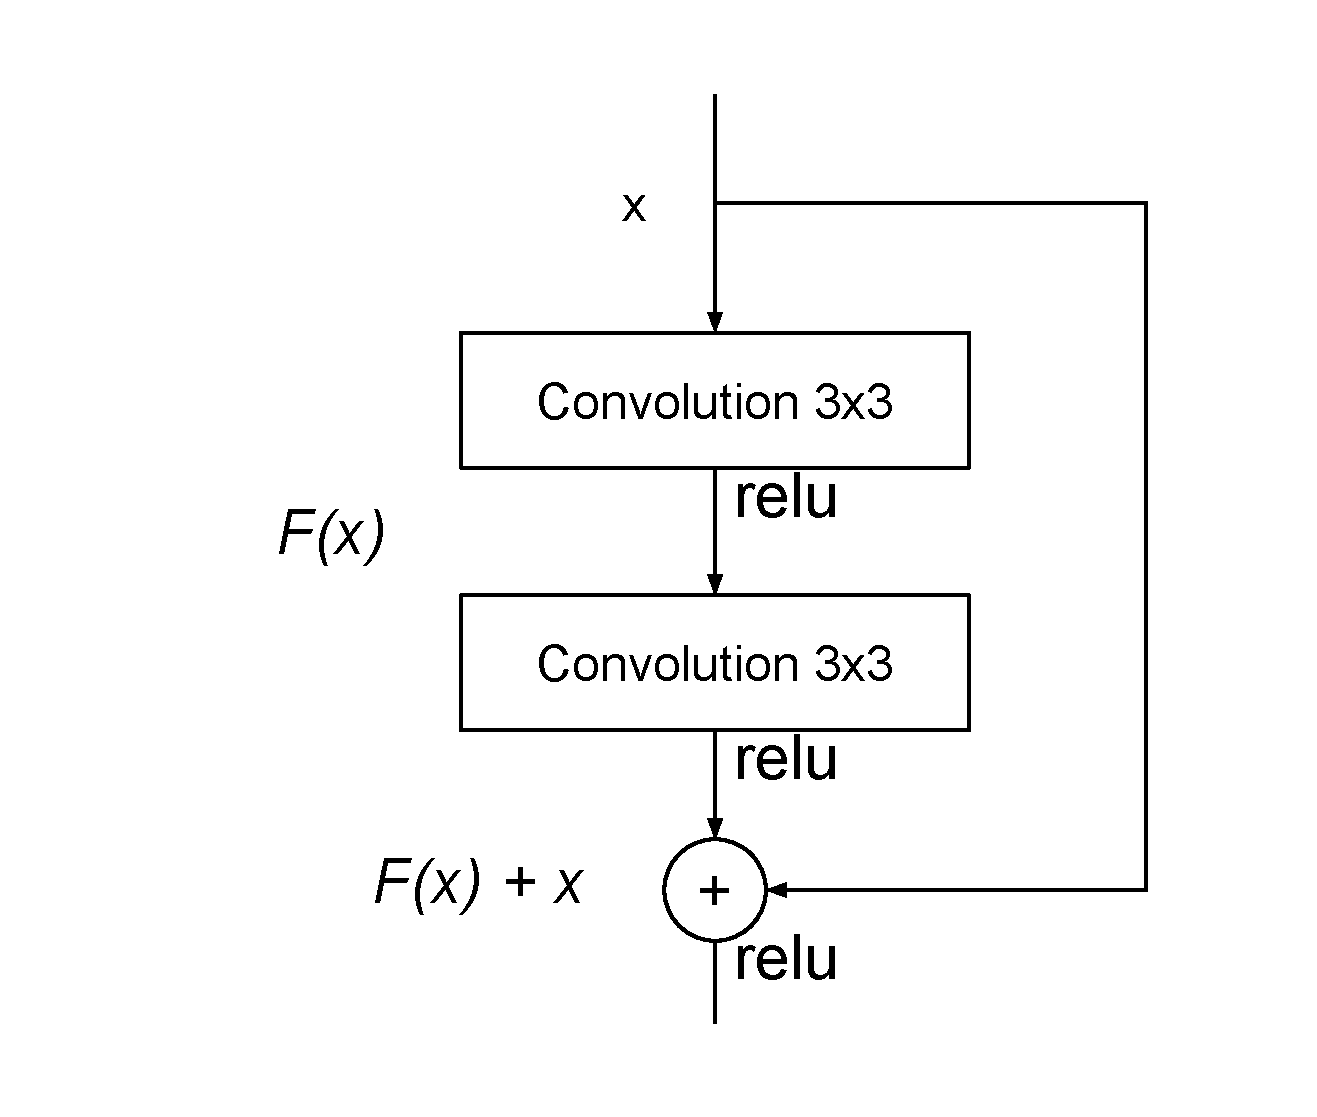
\includegraphics[width=.5\columnwidth]{figures/ResNet.pdf}%
\caption{Exemple d'un bloc résiduel de ResNet (source~\cite{he2015delving}).}%
\label{fig:resnet}%
\end{figure}

Ces connexions résiduelles permettent d'agrandir grandement les réseaux, ainsi l'architecture ResNet présente les meilleurs résultats avec une organisation en 200 couches, avec une erreur sur ImageNet de 4.8\%~\cite{he2016identity}.
Les \textit{skip-connection} peuvent également être utilisées pour connecter le réseau plus densément.
L'architecture DenseNet~\cite{huang2017densely} propose un bloc de base ou chaque couche précédente est connectée aux couches suivantes.
Ces nombreuses nouvelles connections ont plusieurs avantages, notamment de limiter la disparition du gradient, de renforcer la propagation des caractéristiques extraites, et de permettre la réutilisation des caractéristiques extraites précédemment dans le réseau.

Augmenter la taille du réseau ne se fait pas uniquement en profondeur, mais également en largeur.
On peut, dans un bloc, également opérer à plusieurs échelles, en utilisant des convolutions $1*1$, $3*3$ et $5*5$ sur une seule couche.
C'est le cas de l'architecture Inception~\cite{szegedy2015going} qui, pour chaque couche, va multiplier le nombre de convolutions parallèles.
Les architectures suivantes~\cite{szegedy2016rethinking}, jusqu'à InceptionV4~\cite{szegedy2017inception}, reposent sur la même idée d'augmenter la largeur des réseaux, pour travailler à plusieurs échelles sur chaque couche.
Ce type de réseaux a permis de réduire l'erreur sur ImageNet à 3.1\%~\cite{szegedy2017inception}.

\begin{figure}%
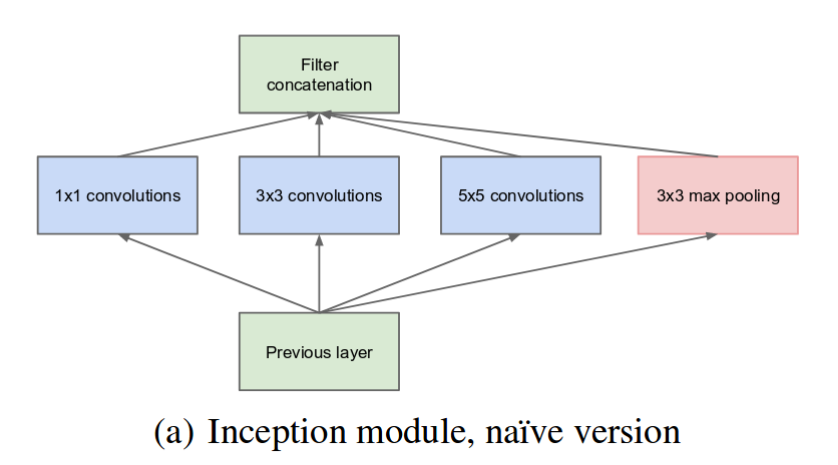
\includegraphics[width=\columnwidth]{figures/inception1.png}%
\caption{Bloc Inception (source~\cite{szegedy2015going}).}%
\label{fig:inception1}%
\end{figure}

Avec l'agrandissement des réseaux, en profondeur et en largeur, la précision sur des tâches de classifications précises comme ImageNet s'améliore~\cite{szegedy2015going, szegedy2016rethinking, szegedy2017inception}.
Cependant, cela mène a des réseaux de plus en plus grands, en terme de mémoire, et de plus en plus lents.
Dans le cas d'une application en mobilité, il n'est pas envisageable d'explorer des réseaux encore plus profonds.
Les architectures présentées précédemment mettent en avant les caractéristiques principales qu'un réseau doit avoir pour obtenir de bon résultats, mais il nous faut viser une diminution de la taille et l'accélération pour garantir des traitements compatibles avec l'interaction d'un humain.



\section{Réduction de la taille et de la complexité des réseaux}
\label{sec:petitsreseaux}

Nous avons présenté des réseaux très profonds, avec de plus en plus de paramètres, pour obtenir des résultats toujours meilleurs.
Le problème étant qu'avec la taille grandissante des réseaux, leur utilisation sur des processeurs mobiles par exemple devient difficile.
Nous nous intéressons dans cette section à des méthodes de réduction de la taille des réseaux, soit par compression, soit en repensant l'architecture, pour que la taille et la rapidité des réseaux deviennent un objectif.


\subsection{Compression des réseaux}
\label{sec:compression}

Une première approche pour la réduction de la taille des réseaux est la suppression des connexions ``inutiles''.
Appelé \textit{pruning}, elle consiste à identifier les connexions inutiles pour les supprimer.
Au début des années 90, cette méthode a beaucoup été étudiée pour réduire la complexité afin de faciliter l'apprentissage~\cite{lecun1989backpropagation, hanson1989comparing, hassibi1993second}, notamment à cause des limitations techniques de l’époque.
Il est possible d'appliquer le \textit{pruning} à des réseaux convolutifs en apprenant quelles connexions sont nécessaires~\cite{han2015learning, han2015deep}.
Les connexions avec des poids faibles, en dessous d'un certain seuil, sont supprimées, et le réseau est ré-entraîné, et ainsi de suite.
Cette approche permet de réduire considérablement le nombre de paramètres, avec par exemple un réduction d'un facteur 9 sur AlexNet et d'un facteur 13 sur VGG.

Il est également possible de réduire la taille en mémoire d'un réseau en réduisant le nombre de bits nécessaires à la représentation de chaque poids.
On peut regrouper les poids à l'aide d'une fonction de hachage~\cite{chen2015compressing}, qui se fait avant l'apprentissage.
En utilisant un algorithme de regroupement, comme k-means~\cite{lloyd1982least}, il est possible de regrouper les poids similaires en un certain nombre de groupes, une fois l'apprentissage réalisé.
Ceci permet de garder les performances du réseau d'origine, et de tirer profit de la redondance dans les réseaux.
La binarisation totale du réseau permet non seulement de grandement réduire la taille du réseau, jusqu'à 32 fois, mais permet surtout l'accélération des calculs, jusqu'à 60 fois~\cite{rastegari2016xnor}. 
Ceci entraîne cependant une diminution logique de la qualité des résultats.


\subsection{Convolutions $1*1$}

Introduit par SqueezeNet~\cite{iandola2016squeezenet}, les réseaux convolutifs avec \textit{micro-architecture} représentent une autre manière de créer des réseaux de tailles réduites.
En créant un réseau de petite taille dès le départ, on peut apprendre le réseau de bout en bout avec moins de paramètres.
Grâce aux dernières avancées sur les réseaux de neurones, notamment les convolutions $1*1$ et les \textit{skip-connections}, on est capable de créer des architectures avec un nombre de paramètres largement réduit, qui arrive à des résultats proches de AlexNet ou VGG~\cite{iandola2016squeezenet, howard2017mobilenets}.

La première stratégie pour réduire le nombre de paramètres est l'utilisation de convolution $1*1$. 
On peut voir ce type de convolution comme une fusion des informations au niveau des pixels, car une convolution regardera le même pixel sur l'ensemble des canaux.
Ce type de convolution utilise logiquement 9 fois moins de paramètres qu'une convolution $3*3$. 
Quelque soit le type de convolution, il est également utile de s'intéresser aux nombre de canaux d'entrée, car ils vont déterminer le nombre de paramètres de la couche.
En combinant des convolutions $1*1$ et des convolutions $3*3$ avec le moins de canaux possibles en entrée, SqueezeNet défini les \textit{fire-modules} (figure~\ref{fig:firemodule}, un type de bloc de convolutions utilisant peu de paramètres.



\begin{figure}%
\centering
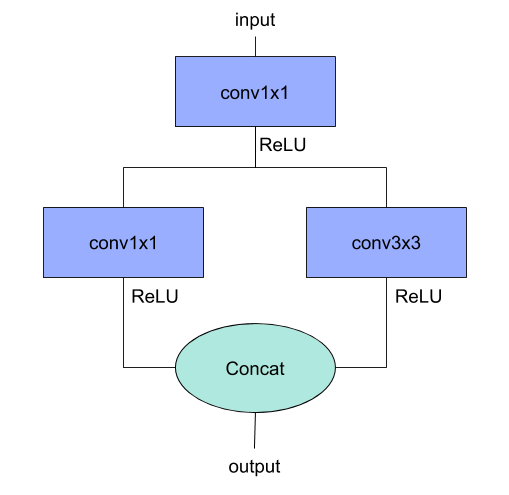
\includegraphics[width=.55\columnwidth]{figures/FireModule.png}%
\caption{Module ``FIRE'' de SqueezeNet~\cite{iandola2016squeezenet}}%
\label{fig:firemodule}%
\end{figure}


Dans le bloc \textit{fire}, la première couche nommée \textit{squeeze} réduit le nombre de canaux pour les convolutions $3*3$ de la deuxième couches pour limiter le nombres de paramètres.
Ce bloc ne réalise pas de sous-échantillonnage, la taille de l'entrée et de la sortie sont donc identiques, seul le nombre de canal va augmenter.
Le sous-échantillonnage est réalisé par des couches de \textit{maxpooling}, assez loin~\footnote{Par ``loin'' on entend ici ``proche de la sortie''.} dans le réseaux, ce qui a tendance à donner de meilleurs résultats, en augmentant la valeur des cartes d'activations~\cite{he2015delving}.
En appliquant ces différentes stratégies, SqueezeNet a des résultats comparables à ceux de AlexNet sur ImageNet, avec un modèle environ 50 fois plus petit.


\subsection{Convolutions groupées}
\label{sec:groupedConv}

Les convolutions groupées~\cite{ioannou2017deep} ont d'abord été introduites pour permettrent de distribuer les calculs pendant l'apprentissage du réseau~\cite{krizhevsky2012imagenet}.
On sépare les canaux en un certain nombre $g$ de groupes, et les convolutions ne vont être utilisées que sur un groupe particulier.
Si l'on a $C$ canaux d'entrée avec $g$ groupes, on a une entrée qui va être composée de groupes de taille $C/g$, où chaque convolution ne va être appliquée que sur un seul de ces groupes.
Comme illustré sur la figure~\ref{fig:groupConv1}, avec un nombre de groupes égal à deux, on divise les convolutions en deux blocs, celle du bloc 1 n'étant effectuée que sur les canaux numérotés $ \left [ 1; C/g \right ] $ n'ayant pas accès aux canaux $ \left ] C/g; C \right ] $

\begin{figure}%

\begin{subfigure}{\textwidth}
	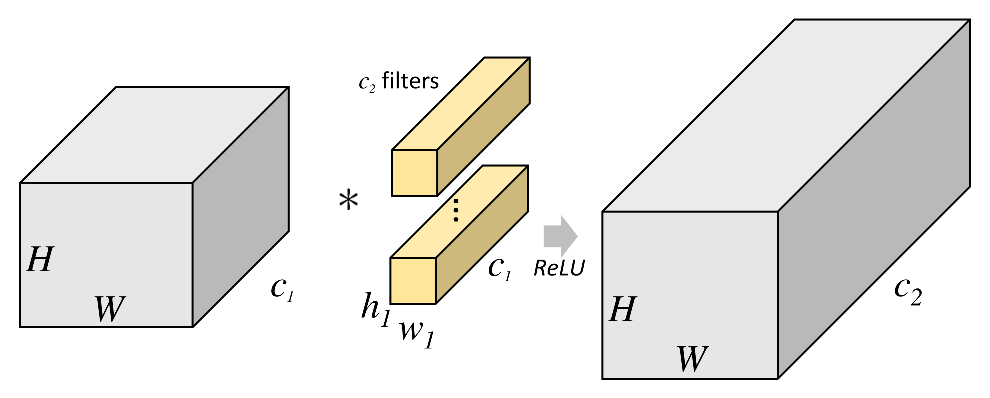
\includegraphics[width=\columnwidth]{figures/convlayer.eps}%
	\caption{Convolution}%
	\label{fig:convsimple1}%
\end{subfigure}

\begin{subfigure}{\textwidth}
	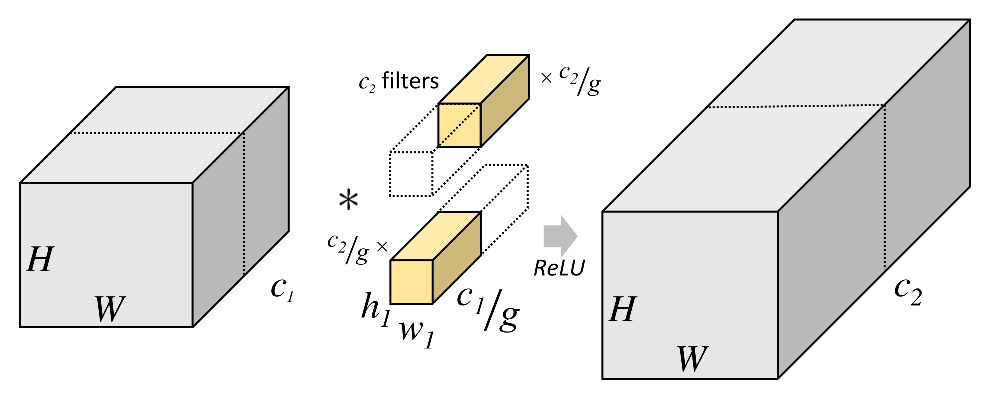
\includegraphics[width=\columnwidth]{figures/filtergroups2.eps}%
	\caption{Convolution avec deux groupes}%
	\label{fig:convsimple2}%
\end{subfigure}

\caption{Illustration des convolutions groupées (source~\cite{ioannou2017deep})}
\label{fig:groupConv1}

\end{figure}

Les convolutions groupées peuvent être apprises séparément (notamment sur plusieurs GPUs) et présentent l'avantage de réduire le nombre de paramètres, avec moins de connexions.
Ces convolutions groupées peuvent être étendues : les \textit{DeepWise Convolution}~\cite{howard2017mobilenets} consiste à prendre un nombre de groupes égale au nombre de canaux en entrée.
Ainsi, chaque canal de sortie n’est connecté qu’à un seul canal d’entrée, comme illustré par la figure~\ref{fig:groupConv}.
Le nombre de paramètres est alors grandement réduit, d'un facteur $C$, mais on perd en contrepartie toute forme d'information entre les canaux.
Pour cela, MobileNet~\cite{howard2017mobilenets} définit un bloc composé d'une convolution \textit{deepwise} $3*3$ et d'une convolution $1*1$ chargé de combiner les informations venant des de chacun des canaux de la convolution \textit{deepwise}.
Ce bloc contient moins de paramètres qu'une convolution $3*3$ classique, et obtient des résultats proches de ceux de VGG~\cite{howard2017mobilenets}, avec en plus l'ajout d'un couche de non-linéarité possible entre les deux convolutions.

\begin{figure}%
\centering
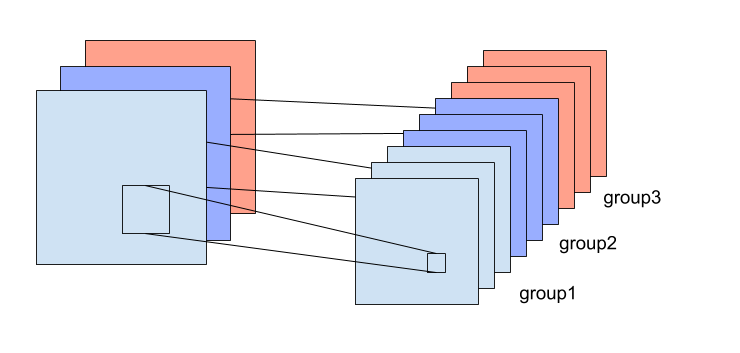
\includegraphics[width=\columnwidth]{figures/groupConvolution.png}%
\caption{Exemple de \textit{DeepWise Convolution}), avec trois groupes pour trois canaux d'entrée.}%
\label{fig:groupConv}%
\end{figure}

L'architecture ShuffleNet~\cite{zhang2017shufflenet} tire profit des deux approches précédentes.
Elle utilise un type de bloc proche de celui de Mobile, mais ajoute une convolution $1*1$ groupée pour réduire le nombre de canaux en entrée de la convolution $3*3$.
La convolution $1*1$ de fusion des informations est remplacée par une convolution $1*1$ groupée (figure~\ref{fig:shufflemodule}). 
Mais pour que celle-ci ait quand même un rôle de fusion d'information, une opération de mélange des canaux est réalisée entre les deux convolutions, en plus d'ajouter une \textit{skip-connection}.
Cette approche permet d'obtenir des résultats légèrement supérieurs à MobileNet, mais avec environ $4.5$ fois moins de paramètres grâce aux convolutions groupées.


\begin{figure}%
\centering
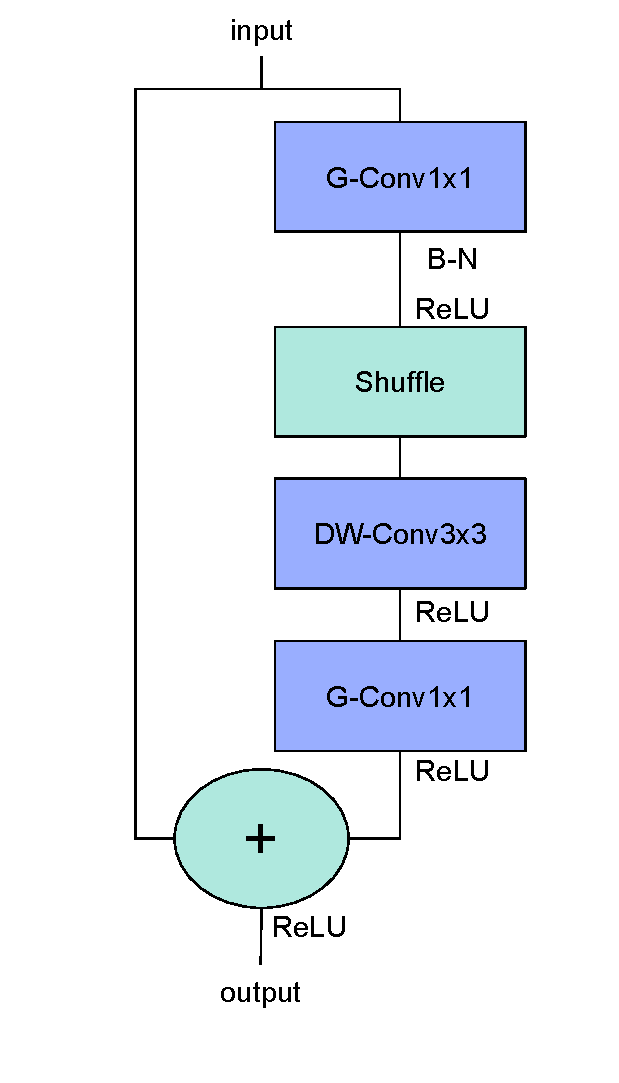
\includegraphics[width=.35\columnwidth]{figures/ShuffleModule.pdf}%
\caption{Module ``Shuffle'' de ShuffleNet~\cite{zhang2017shufflenet}}%
\label{fig:shufflemodule}%
\end{figure}

Ces différentes micro-architectures permettent d'obtenir des résultats proches ou parfois supérieurs aux réseaux profonds avec des millions de paramètres sur des tâches comme ImageNet.
Ils montrent surtout différentes stratégies de réduction des architectures intéressantes.
Dans le chapitre~\ref{chap:gestes}, nous nous intéressons à un réseau de petite taille adapté à une application en mobilité, et utilisons ces différentes méthodes pour construire un réseau adapté à la reconnaissance de gestes. 


\section{Réseaux avec détection de régions}
\label{sec:rpn}

L'utilisation des réseaux de neurones convolutifs n'est pas limitée à la classification des images, et des méta-architecture permettent par exemple leur utilisations pour la détection des régions d'intérêt sur les images. 
Par méta-architecture, nous entendons une architecture construite autour d'une architecture précédemment définie, comme celles que nous avons présentées dans la section~\ref{sec:cnn}.
En utilisant un réseau appris à reconnaître un certain nombre d'objet, il est possible détecter où cet objet se situe dans l'image.
Pour cela on distingue deux types d'approches, avec des réseaux à proposition de régions (section~\ref{sec:propositionderegions}) , ou à l'aide de carte d'activation (section~\ref{sec:cartedactivation}).


\subsection{Proposition de régions}
\label{sec:propositionderegions}

Il est possible de faire apprendre directement à un réseau les régions d'intérêt sur les images, si l'on dispose d'un corpus d'apprentissage avec les régions annotées.
Des collections d'images comme MS COCO~\cite{lin2014microsoft} proposent un grand nombre d'images avec des boîtes englobantes autour des objets.
Ceci permet de construire un réseau qui va à la fois classifier image et proposer une région pour la localisation de l'objet.
Les réseaux de type R-CNN (pour Region Convolutional Neural Network)~\cite{girshick2014rich} permettent de créer de proposer des boîtes englobantes pour les objets présents dans l'image.
La proposition Fast-RCNN~\cite{girshick2015fast}, présentée sur la figure~\ref{fig:fastrcnn}, consiste à permettre au réseau de produire deux sorties, une de classification, et une de région d'intérêt. 
Le réseau apprend à produire la boîte englobante correspondant à celle donnée par le corpus d'apprentissage, et à classifier uniquement cette zone.

\begin{figure}%
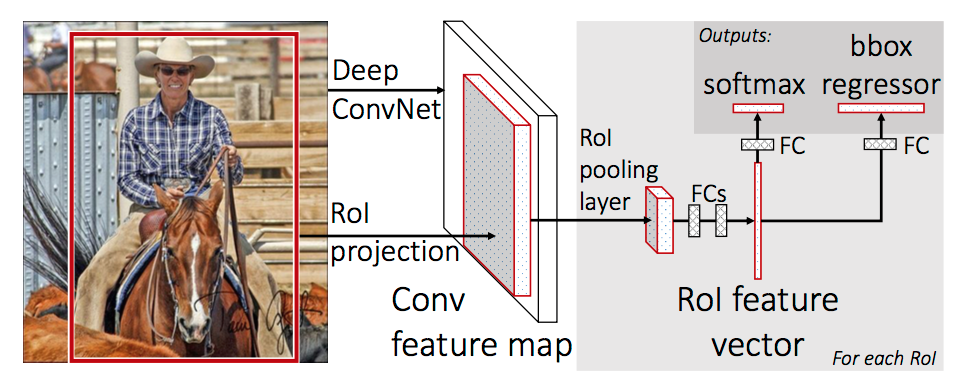
\includegraphics[width=\columnwidth]{figures/fast-rcnn.png}%
\caption{Architecture Fast-RCNN~\cite{girshick2015fast}}%
\label{fig:fastrcnn}%
\end{figure}

L'approche Faster-RCNN~\cite{ren2015faster} ajoute un \textit{Region Proposal Network} après la dernière couche de convolution.
Ce réseau est capable de regarder les caractéristiques de la dernière couche de convolution pour déterminer une région d'intérêt probable.
Ensuite, la même méthode de classification que cette de Fast R-CNN 



\subsection{Cartes d'activations}
\label{sec:cartedactivation}

Il a été montré que les réseaux convolutifs étaient capables de détecter les objets dans une images même si l'apprentissage s'est fait sur des images entières, sans indications sur la présence des objets.
Avec un réseau entrainé sur ImageNet, en regardant où se situe les maximum d'activation dans le différents filtres de convolutions, on remarque ceux-ci se concentre sur l'objet à reconnaître~\cite{le2013building}.
Mais surtout, entraîné à reconnaître des scènes, comme des pièces ou des lieux extérieurs, on note des activations sur des objets bien particuliers (lampes, lits, etc) alors qu'aucune information sur ces objets n'a été fournie au réseau~\cite{zhou2014object}. 
Ceci sous entend que le réseau a bien une représentation interne de ces objets, lui permettant de les reconnaître, et de reconnaître les scènes.
Toutefois, ces informations de localisation sont perdues avec l'utilisation de couches entièrement connectées.
En effet, ces couches utilisées pour la classification fusionnent les informations venant de tous les canaux, et la localisation des objets devient impossible.
Il est cependant possible d'extraire l'information avant qu'elle ne passe à travers les couches entièrement connectées, pour ainsi avoir deux formes de sorties, une qui indique la position de l'objet, et l'autre qui indique sa classe~\cite{zhou2016learning}.
Néanmoins, ceci ne permet pas de faire un apprentissage de ces régions et les zones d'activations ne correspondent pas forcément à ce qui est classifié, comme on ne tient pas compte de l'information présente dans les couches de classification pour savoir ce qui est important où non pour telle ou telle classe.

Un autre manière d'obtenir une carte d'activation est d'utiliser une image plus grande, de la séparer en sous-régions, et de classifier chacune des régions.
En plus d'être très coûteuse, car il faut appliquer le réseau une fois pour chaque pixel de la carte d'activation, un réseau composé uniquement de convolutions réalise la même opération.
Les \textbf{réseaux entièrement convolutifs}, c'est-à-dire sans aucune couche entièrement connectée, présentent deux principaux avantages : ils permettent de garder des informations sur l'organisation spatiale de l'image sur l'ensemble du réseau, et ils peuvent être appliqués facilement sur n'importe quelle taille d'image étant donné qu'ils ne sont composé que de convolutions.
Il est possible de transformer une couche entièrement connectée en une convolution $1*1$, comme le type d'opération est similaire, avec les mêmes paramètres~\cite{long_fully_2015}.

\begin{figure}%
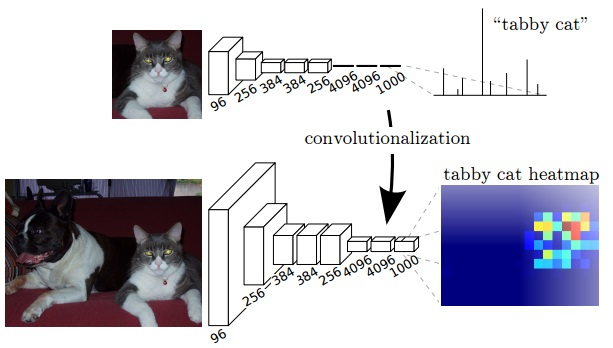
\includegraphics[width=\columnwidth]{figures/FCN.jpg}%
\caption{Transformation d'une couche entièrement connectée en convolution pour obtenir une carte d'activation~\cite{long_fully_2015}}%
\label{fig:convolutionalisation}%
\end{figure}

La sortie d'un réseau entièrement convolutif représente, comme dans un réseau classique, la probabilité de classification pour chaque classe.
Cependant, un réseau de neurones à un \textbf{champ de réception} limité, c'est-à-dire qu'il ne regarde que sur une image d'une dimension donnée.
En appliquant un réseau entièrement convolutifs, on peut l'appliquer sur une image de dimension arbitraire.
Ainsi, plus l’image d’entrée est grande, plus la sortie est grande.
On peut ainsi interpréter la sortie comme une carte d'activation du réseau sur l'image (figure~\ref{fig:convolutionalisation}).

En ajoutant des connexions entre l'entrée et la sortie, ou en utilisant une base de données avec des informations sur les régions d'intérêt, il est possible d'apprendre plus précisément cette carte d'activation~\cite{long_fully_2015}.
Même si ces méthodes ne permettent pas d'obtenir des régions d'intérêt, mais uniquement des zones d'activation, elles ont l'avantage de ne pas nécessiter d'apprentissage particulier sur des corpus avec des régions annotées.
C'est un point important dans notre cas, et dans le chapitre~\ref{chap:regions}, nous utilisons ces réseaux entièrement connectés pour nous aider dans la détection des œuvres. 



\section{Identification d'instances}
\label{sec:stateidentification}

La recherche d'instances est une tâche de recherche visuelle qui vise, à une image de requête, à récupérer toutes les images qui contiennent la même instance d'objet dans une base de données d'images. 
La recherche d'instances a une large gamme d’applications, comme par exemple la recherche inversée d’image sur le web ou l'organisation de collections de photos personnelles.
Dans notre cas, nous utilisons la recherche d'instances pour réaliser l'identification d'oeuvres avec le dispositif GUIMUTEIC.

Malgré les avancées récentes des réseaux de neurones que nous avons présentées précédemment, ils sont resté longtemps en deçà des méthodes à bases de descripteurs visuels pour la recherche d'instances~\cite{mikulik2013learning, tolias2014visual}.
Les approches modernes basées sur l'apprentissage de similarité et l'apprentissage de classement (learning to rank) permettent d'obtenir les meilleurs résultats aujourd'hui~\cite{gordo2016deep}.

\subsection{Caractéristiques ingéniérées}
\label{sec:ingeniere}

La recherche de similarité entre les images a longtemps été basée sur la correspondance entre les descripteurs visuels extraits des images.
Un descripteur visuel capture une caractéristique d'un point de l'image.
Dans le cas idéal, cette description doit être invariante à l'orientation, à l'échelle, aux différences de prise de vue, etc.
Les méthodes d'extraction de descripteurs se basent sur la détection de points clefs de l'image, l'extraction de caractéristique de chacun de ces points, pour finalement représenter l'image par l'ensemble de ces descripteurs.
La qualité de la représentation de ces images va être dépendante de deux éléments principaux : si les points clefs représentent bien l'image et si l'extraction de caractéristique permet de capturer suffisamment d'information.

Le descripteur SIFT (Scale Invariant Feature Transform) développé par Lowe~\cite{lowe1999object} présente de très bon résultats notamment pour la reconnaissance d'objet~\cite{lowe2004distinctive, ferrari2004simultaneous, mikolajczyk2005performance, karami2017image} ou la recherce d'image~\cite{mikolajczyk2001indexing}.
SIFT combine un détecteur de régions invariant à échelle (par différence de gaussiennes) et un descripteur basé sur la distribution de gradient dans les régions détectées.
Cependant, il nécessite une grande complexité de calcul, ce qui est un inconvénient dans notre cas, et en général dans les applications en temps réel~\cite{lowe2004distinctive, juan2009comparison}. 


De nombreuses variantes à SIFT existent pour régler certains problèmes, notamment la vitesse de calcul~\cite{chiu2013fast}, ou la précision du descripteur~\cite{ke2004pca}.
Speed Up robust Features (SURF) est une approximation de SIFT, qui  est plus rapide, sans réduire la qualité des points détectés~\cite{bay2008speeded}.
Les descripteurs BRIEF (Robust Indépendant Elementary Features) proposent une alternative aux descripteurs de SIFT, beaucoup moins complexe, avec une précision d'appariement entre les descripteurs très proche~\cite{calonder2010brief}.
Dans le but de viser les appareils mobiles, le descripteur ORB (Oriented FAST and Rotated BRIEF)~\cite{rublee2011orb} couple le détecteur de points clefs FAST~\cite{rosten2006machine}, qui est plus rapide que les différences de gaussienne de SIFT, avec le descripteur BRIEF.
Ce dernier descripteur permet d'avoir une solution utilisable sur processeur mobile, avec des performances proches de celle de SIFT~\cite{rublee2011orb}.

Dans le cadre de la recherche d'image, ou l'identification d'instances, la plupart des méthodes à base de descripteurs visuels utilisent le même type d'approche : l'image est représentée par un certain nombre de descripteurs, qui sont regroupés en un vecteur ou un ensemble de vecteurs, et on compare l'image requête à l'ensemble des images de la base de données grâce à ces vecteurs.
A la manière des sacs de mots en recherche d'information textuelle, on peut regrouper ces descripteurs en sac de mots visuels~\cite{sivic2003video}, ce qui les rend compatible avec les fichiers inverses~\cite{zhang2011image}, avec des représentations binaires ou compactes~\cite{nister2006scalable,philbin2007object,jegou2008hamming}, avec les Fisher Vector~\cite{perronnin2010large}, les VLAD~\cite{jegou2010aggregating} ou avec l'ajout d'extension de requêtes~\cite{chum2007total, arandjelovic_three_2012}. 
Les descripteurs visuels permettent également une vérification géométrique pour la vérification des résultats de correspondance entre les descripteurs~\cite{philbin2007object, perd2009efficient}.
Cependant, les solutions à base de réseaux de neurones présentent aujourd'hui les meilleurs résultats et proposent de nombreuses solutions adaptées~\cite{zheng2018sift}.


\subsection{Extraction de caractéristiques}
\label{sec:extractfeatures}

Il a été présenté par Krizhevsky et al.~\cite{krizhevsky2012imagenet} qu'extraire des caractéristiques de l'image depuis les couches cachées d'un réseau de neurones pourrait remplacer les descripteurs ingéniérés, ce qui sera prouvé plus tard par de bons résultats pour pour la recherche d'instances~\cite{sharif2014cnn}.
Il est en effet possible d'utiliser tout ou une partie d'un réseau de neurones sur une tâche différente de laquelle il a été entraîné.
Comme montré dans les sections précédentes, un CNN typique se compose de plusieurs couches convolutionnelles, suivies de couches entièrement connectées et se termine par une couche SoftMax produisant une distribution de probabilité sur les différentes classes. 
Au lieu d’utiliser ce classificateur intégré, il est possible de considérer les activations des couches intermédiaires comme représentation d'image, comme montré sur la figure~\ref{fig:extractfeatures}.
Il est ainsi possible d'utiliser un autre classifieur sur cette nouvelle sortie du réseau, sur une tâche complètement différente de celle de départ, avec pourtant de bons résultats~\cite{oquab2014learning}.


\begin{figure}[ht!]
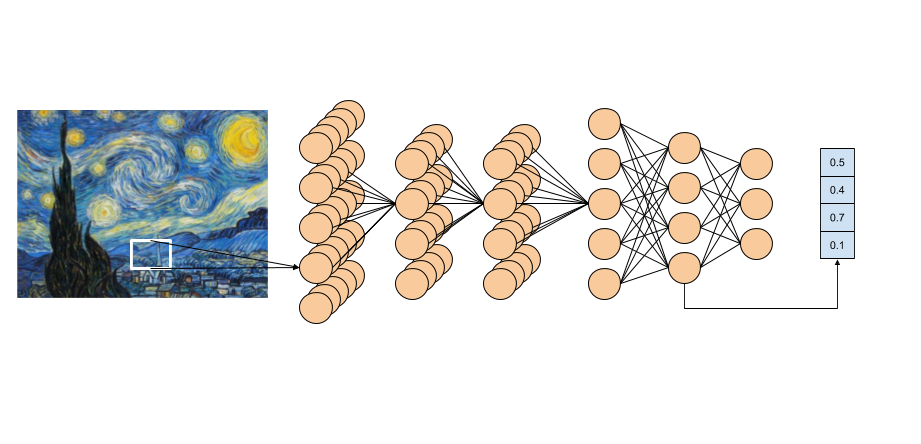
\includegraphics[width=\columnwidth]{figures/ExtractFeatures.png}%
\caption{Exemple d'extraction de caractéristiques depuis une couche cachée d'un réseau de neurones.}%
\label{fig:extractfeatures}%
\end{figure}


Ces représentation d'images ``apprises''~\footnote{On parle de représentation d'image apprise car elle est issue d'un réseau de neurones entraîné. Elle n'est cependant pas forcément adapté à la tâche sur laquelle elle est utilisé.} permettent d'obtenir des résultats parfois meilleurs que les descripteurs ingéniérés~\cite{sharif2014cnn}.
Cependant, elles souffrent d'un manque de robustesse à l'orientation, à la mise à l'échelle ou au bruit, ainsi que de l'impossibilité de les régler précisément pour une tâche, les rendent moins performants.
Les travaux récents montrent que l'utilisation des sorties des couches intermédiaires plutôt que des dernières couches entièrement connectées donnent de meilleurs résultats. Particulièrement lorsque l'on s'intéresse aux objets dans les images, notamment grâce à une plus grande généralité des caractéristiques, moins spécialisées sur la tâche apprise~\cite{donahue2014decaf, azizpour2015generic}.

Plusieurs améliorations ont été proposées pour palier à leur manque de robustesse, notamment à base de régions sur les images.
En utilisant les sorties du réseau de neurones sur un certain nombre de régions de l'image, on obtient une description des régions, qu'il est possible d'accumuler~\cite{babenko2015aggregating, sharif2015baseline, kalantidis2016cross, tolias2015particular}, ou d’agréger en Fisher Vector~\cite{perronnin2015fisher} ou avec des VLAD~\cite{gong2014multi, paulin2015local}.
L'avantage de l'utilisation des régions est qu'une vérification géométrique est possible lorsque l'on compare deux images, et que le ratio des images peut être conserver, ce qui évite les déformations~\cite{tolias2015particular, gordo2016deep}.
Cependant, l'utilisation de caractéristiques issues d'un réseau entraîné sur une collection standard, généralement ImageNet, ne peut pas garantir qu'elles soient adaptées à la tâche qui nous intéresse.

Lorsque l'on travaille sur des collections de recherche d'images, il n'est généralement pas possible d'entraîner un réseau de neurones profonds complet sur celles-ci, car il y a un nombre de classes très grand pour un nombre d'exemples très limité, en plus d'une faible variabilité entre les images d'exemple.
La plupart des méthodes présentées précédemment utilisent un réseau pré-entraîné sur ImageNet ou autre grande collection.
On peut réaliser un réaliser un fine-tuning (voir encadré et figure~\ref{fig:finetuning}) sur la collection de recherche d'image, et malgré des résultats qui ne sont généralement pas suffisants pour permettre une bonne classification des images, ce fine-tuning améliore les résultats de l'extraction de caractéristiques~\cite{babenko2014neural, gordo2016deep, radenovic2016cnn}

\begin{oframed}
\textbf{Fine-tuning} : On entend par fine-tuning (ou apprentissage fin) le fait de remplacer la dernière couche de classification d'un réseau appris sur une tâche donnée par une nouvelle et d'entraîner tout ou un partie du réseau sur cette nouvelle tâche. Cette méthode est généralement utilisée lorsque l'on doit travailler sur des collections insuffisamment grandes ou variées pour qu'un réseau profond soit appris.
\end{oframed}


\begin{figure}[ht!]
\centering
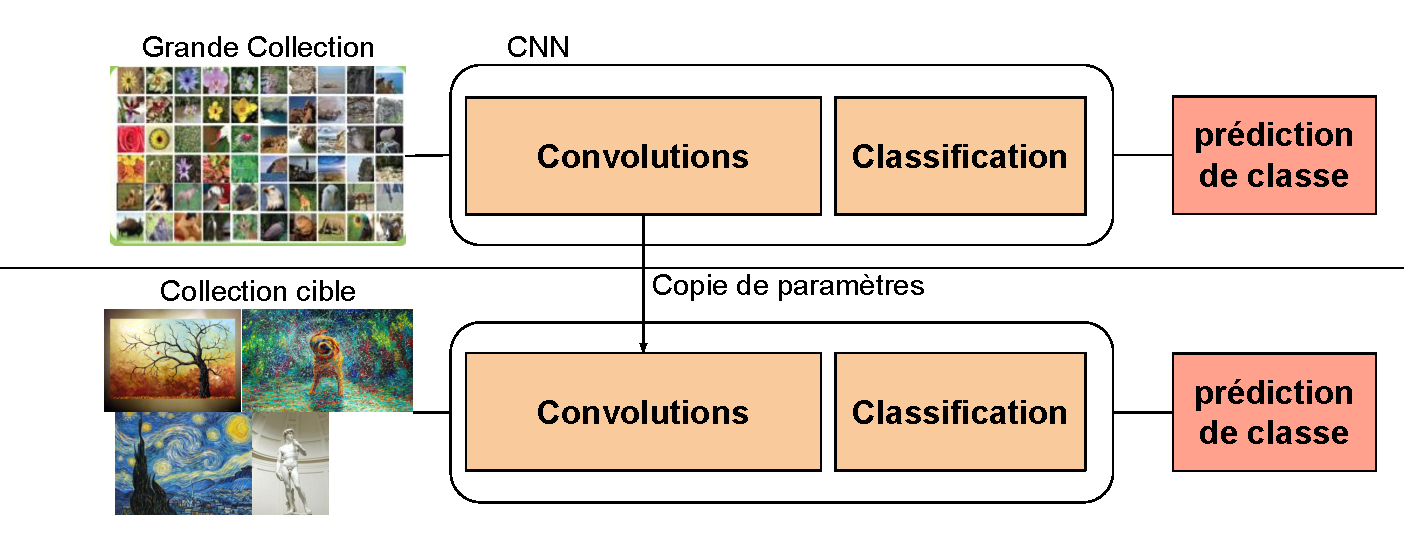
\includegraphics[width=\columnwidth]{figures/finetuning.pdf}%
\caption{Illustration du fine-tuning, avec apprentissage sur première collection et second apprentissage sur la collection cible.}
\label{fig:finetuning}
\end{figure}

La figure~\ref{fig:histoire}, tirée de~\cite{zheng2018sift}, retrace la chronologie des recherches présentées précédemment.
On remarque l'entrée dans l'ère du CNN, pour citer l'auteur, avec d'abord l'extraction de caractéristiques globales depuis un réseau pré-traîné, jusqu'à la représentation de régions par Tolias et al.~\cite{tolias2015particular}.
Cette chronologie s'arrête en 2016, avec un nouveau changement de paradigme, qui est l'arrivé des réseaux siamois, notamment avec l'arrivé de FaceNet~\cite{schroff2015facenet}.


\begin{figure}%
\centering
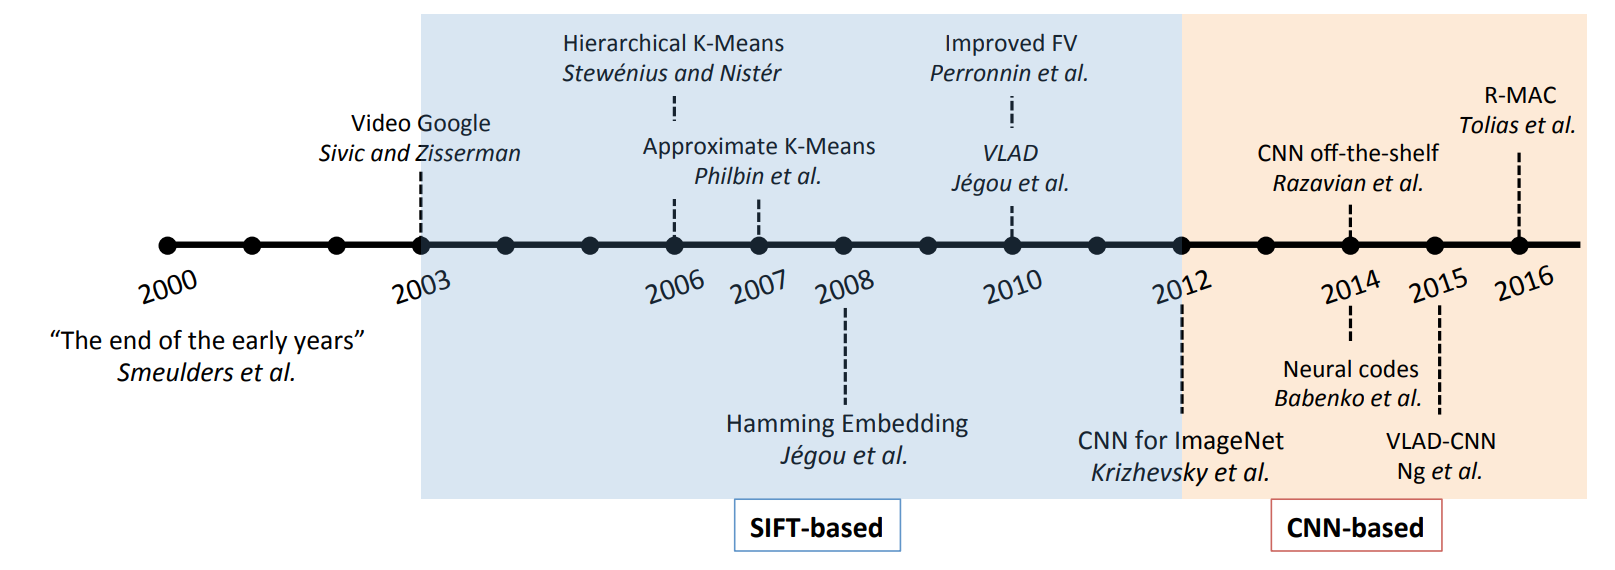
\includegraphics[width=\columnwidth]{figures/histoireRI.jpg}%
\caption{Chronologie sélective de la recherche d'instance (source~\cite{zheng2018sift}).}
\label{fig:histoire}
\end{figure}

\subsection{Apprentissage de similarité}
\label{sec:transfertlearning}

Les réseaux siamois~\cite{baldi1993neural, bromley1994signature} ont été introduits pour résoudre le problème de comparaison entre deux images.
Le réseau proposé par~\cite{bromley1994signature} est montré sur la figure~\ref{fig:siamois}.
Il s'agit d'utiliser deux fois le même réseau, avec deux entrées différentes.
On présente alors au réseau un ensemble de couples, des paires d'images représentant le même objet ou non.
Les deux sorties du réseau sont alors comparé, et l'apprentissage se fait par rétro-propagation~\cite{lecun1989backpropagation} sur les deux branches. 

\begin{figure}%
\centering
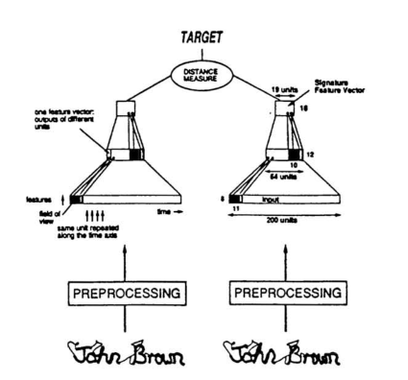
\includegraphics[width=\columnwidth]{figures/siamese.png}%
\caption{Réseau siamois présenté par~\cite{bromley1994signature}}
\label{fig:siamois}
\end{figure}

L'avantage de ce type de méthode est que l'apprentissage correspond à la tâche pour laquelle le réseau est utilisé, contrairement aux approches de la section précédente.
Il est alors possible d'entraîner un réseau à produire une projection des images qui correspond à la problématique qui nous intéresse.
Par exemple, si la taille de sortie du réseau est de dimension $N$, et que l'on compare les sorties de chacune des deux branches du réseau avec une distance (euclidienne ou autre), il est possible d'apprendre au réseau à projeter les images dans cet espace de dimension $N$ pour que la distance entre les projections représente la similarité entre les images.
Soient $I_1$ et $I_2$ deux images, et $\hat{x}$ qui vaut 0 si les images représentent le même objet, 1 sinon. 
L'équation~\ref{eq:coupleloss} montre une fonction de coût possible associé au réseau siamois, avec $F(x)$ la sortie d'une branche du réseau pour l'entrée $x$.

\begin{equation}
L(I_1, I_2, \hat{x}) = (1-\hat{x})*||f(I_1)-F(I_2)||_2^2 + \hat{x}*max(0,m-||f(I_1)-F(I_2)||_2^2)
\label{eq:coupleloss}
\end{equation}

Le résultat de cette équation est différent de 0 dans les cas suivants :
\begin{itemize}
	\item $\hat{x}$ = 0 et la distance $||f(I_1)-F(I_2)||_2^2$ est supérieure à 0.
	\item $\hat{x}$ = 1 et la distance $||f(I_1)-F(I_2)||_2^2$ est inférieure à une marge $m$ fixée.
\end{itemize}

Il faut alors, dans ces cas, mettre à jour le réseau par rétropropagation. 
Autrement dit, on entraine le réseau à produire une projection $f$ tel que les images similaires soient projetées sur le même point, et que les images différentes aient une projection séparée d'une marge $m$.
Ainsi, pour la recherche d'instances, nous pouvons parcourir l'ensemble des images de la base de donnée et trouver les images avec une projection identique pour déterminer l'objet présent dans l'image requête.

FaceNet~\cite{schroff2015facenet} propose d'utiliser les réseaux siamois pour comparer les visages dans les images.
En utilisant cette fois-ci un réseau à trois branches, les entrées sont un ensemble de triplets plutôt que de couples.
Les triplets sont composés d'une image de base (appelée \textit{anchor}), d'une image représentant la même instance (appelée \textit{positive}) et une image différente (appelée \textit{negative}).
L'objectif est alors de produire une projection par le réseau, telle que la représentation de l'image \textit{anchor} soit plus proche de l'image \textit{positive} que de l'image \textit{negative}.
On peut alors définir une nouvelle fonction de coût, avec les images $I_a$, $I_p$ et $I_n$ respectivement anchor, positive et négative.
L'équation~\ref{eq:facenetloss} va alors être positive lorsque $||f(I_a)-F(I_p)||_2^2 > ||f(I_a)-F(I_n)||_2^2$, et elle vaudra 0 lorsque $f(I_a)$ sera plus proche de $f(I_p)$ que de $f(I_n)$, comme montré sur le schéma~\ref{fig:facenet}, pris depuis~\cite{schroff2015facenet}.

\begin{equation}
L(I_a, I_p, I_n) = max(0, ||f(I_a)-F(I_p)||_2^2 - ||f(I_a)-F(I_n)||_2^2)
\label{eq:facenetloss}
\end{equation}

\begin{figure}%
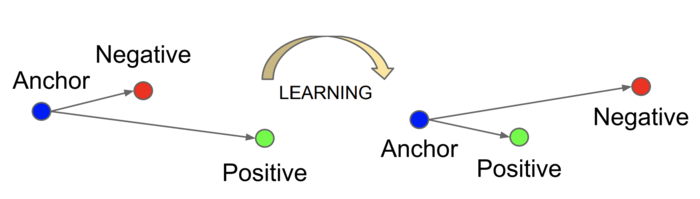
\includegraphics[width=\columnwidth]{figures/facenet.png}%
\caption{Apprentissage des projection avec un réseau triple (source~\cite{schroff2015facenet})}%
\label{fig:facenet}%
\end{figure}

La figure~\ref{fig:tripletloss} présente l'apprentissage d’un réseau siamois à trois branches.
La première image en haut à gauche est l'image de base, la seconde l'exemple positif et la troisième l'exemple négatif.
Le réseau de neurones (CNN) est présenté trois fois sur le schéma, mais il s'agit bien du même réseau. 
Les poids sont partagés entre les branches, et l'apprentissage est fait simultanément, le réseau est donc bien toujours le même sur les trois branches.

\begin{figure}[ht!]
	\centering
    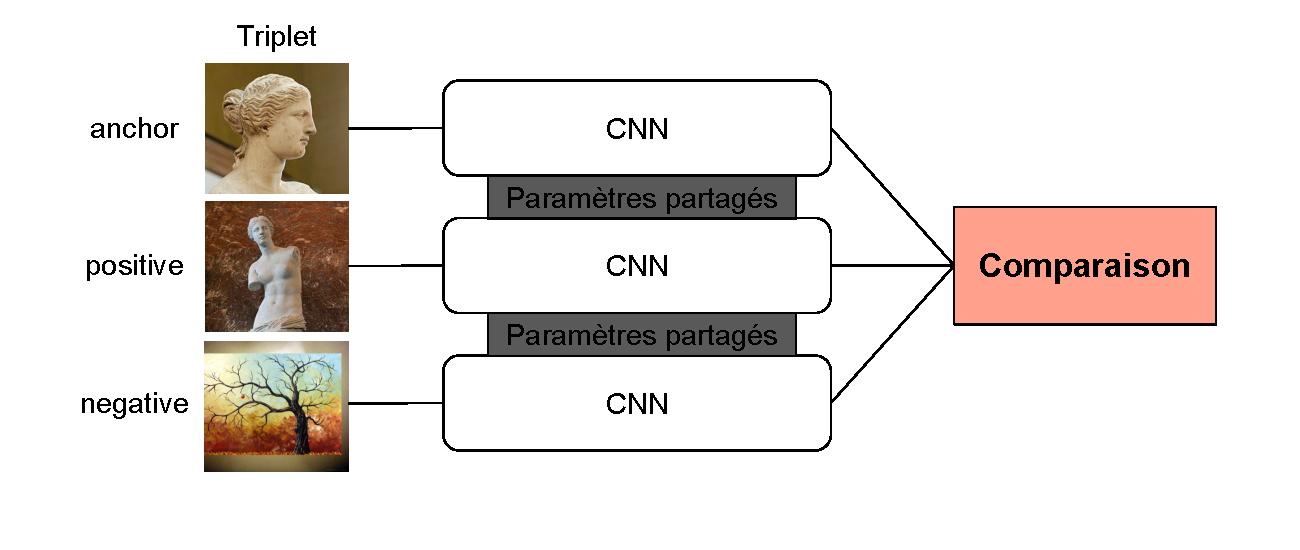
\includegraphics[width=\linewidth]{figures/3branches.pdf}
    \caption{Réseau siamois à trois branches}
		\label{fig:tripletloss}
\end{figure}

Schroff et al.~\cite{schroff2015facenet} mettent également en avant le problème de sélection des triplets, qui a un rôle très important dans la capacité à entraîner le réseau. 
Cette problématique est très dépendante des corpus sur lesquels est entraîné le réseau et dans le chapitre~\ref{chap:similarite} nous abordons ce problème dans le cadre de nos collections.

Gordo et al.~\cite{gordo2016deep} se basent sur l’approche de Schroff et al. et sur celle de Tolias et al.~\cite{tolias2015particular}, pour enrichir cette architecture avec une proposition de régions d'intérêts.
En utilisant la projection d'une région d'intérêt plutôt que de l'image entière, ils sont capable de produire une projection qui capture mieux la similarité entre les objets.
Nous nous basons notamment sur leur approche pour proposer notre propre architecture dans le chapitre~\ref{chap:regions}.

Les réseaux siamois à trois branches sont particulièrement bien adaptés à la recherche d'instances.
Ils obitennent en effet les meilleurs résultats sur les collections courante de recherche d'instance~\cite{gordo2016deep}.
Dans les chapitres~\ref{chap:similarite} et~\ref{chap:regions}, nous les explorons plus en détail et nous étudions comment les adapter à notre problème, tout en proposant une nouvelle fonction de coût et un nouveau pipeline d'apprentissage.


\section{Détection d'événement dans les vidéos}
\label{sec:stateVideo}

Dans le cadre du projet GUIMUTEIC, en plus de la partie reconnaissance d'instance, nous nous intéressons à la reconnaissance de gestes dans les vidéos.
Nous avons mis en évidence 5 gestes (6 si l'on ajoute la détection de l'absence de geste), qu'il faut identifier (section~\ref{sec:gestesGUIMUTEIC}).
L'approche standard de la classification vidéo comporte trois étapes principales~\cite{sivic2003video, liu2009recognizing, wang2009evaluation}, qui est très proche de celle présentée précédemment sur la classification d'image :

\begin{itemize}
	\item Extraction de caractéristiques visuelles locales avec des descripteurs visuel, qui en plus de ceux présentés précédemment peuvent être temporelles~\cite{dollar2005behavior,wang2011action}.
  \item Création d'une description pour chaque segment de vidéo, par exemple à l'aide de sac de mots visuels~\cite{laptev2008learning}.
	\item Entraînement d'un classifieur (SVM généralement) pour la reconnaissance d'actions.
\end{itemize}

Ce pipeline a les mêmes désavantages que ceux présenté dans la section~\ref{sec:ingeniere}, et le fait qu'ils se basent sur des descripteurs ingéniérés est l’une des limitations principales.
Les premières application de CNN pour la détection d'action dans les vidéos consiste à considérer l'entrée comme une image avec une dimension de plus (le temps), et d'appliquer des convolutions 3D à la place des convolutions 2D présentées précédemment.
Une convolution 3D est similaire à une convolution 2D, et l'architecture utilisée est alors similaire à celle d'un réseau profond type AlexNet~\cite{baccouche2011sequential}.
Les caractéristique visuelles spatiales et temporelles sont donc considérées de la même manière.
D'autres approches proposent de traiter différemment les données spatiales et temporelles avec deux réseaux distincts~\cite{simonyan2014two}, avec un réseau qui s'intéresse uniquement à l'image et l'autre qui regarde le flux optique de la vidéo.
Le principal problème ici vient du fait qu'il faut calculer le flux optique pour chaque image de la vidéo, et dans un contexte mobile cela se révèle très coûteux, et rédhibitoire pour une application en temps réelle.

Karpathy et al.~\cite{karpathy2014large} proposent de traiter les données temporelles à l'intérieur du réseau de neurones.
La figure~\ref{fig:videofusion} présente différentes manières de réaliser la fusion des information des informations temporelles, avec en bas la série temporelle d'image composant la vidéo et en haut la classification issue du réseau.
Le \textit{single frame} correspond à faire de la classification d'image classique comme présenté précédemment.
Ne prenant en compte aucune donnée temporelle, il s'agit de celui qui donne les moins bons résultats, et sert généralement de baseline.
La \textit{late fusion} prend deux trames, les fait passer chacune dans le réseau et, grâce aux couches entièrement connectées finale, faire une fusion.
Le désavantage principal de cette technique est l'augmentation du temps de calcul, avec chaque trame lu devant être passer dans le réseau.
De plus, tout le travail de fusion est réalisé par une couche entièrement connectée, ce qui fait beaucoup de paramètres supplémentaire, avec une solution optimale potentiellement plus difficile à trouver.
La \textit{early fusion} consiste à considérer l'entrée non plus comme une image, mais comme une matrice de dimension 3, ce qui revient à concaténer les images images à la suite les unes des autres en entrée.
L'avantage principal est le nombre de paramètres du réseau qui n'augmente que très peu, mais le problème vient de la perte rapide d'information temporelle.
Enfin la \textit{slow fusion} présente les meilleurs résultats, et propose de fusionner les informations temporelles au fur et à mesure dans le réseau.
Cette technique est une intégration des deux précédente, en prenant leurs avantages respectifs, sans les inconvénients.

\begin{figure}[ht!]
\centering
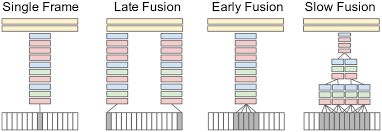
\includegraphics[width=\columnwidth]{figures/videofusion.png}%
\caption{Différentes méthodes de fusion d'information temporelle avec un CNN (source~\cite{karpathy2014large}).}
\label{fig:videofusion}
\end{figure}

Ce type d'approches cependant est généralement dépassé en terme de performance par des réseaux récurrents (RNN)~\cite{donahue2015long}.
Ce type de réseau connecte chaque entrée aux entrées précédentes, ce qui lui permet de garder une ``mémoire'' des informations passées.
Sur la figure~\ref{fig:rnn}, on voit une représentation simplifiée d'un tel réseau récurrent.
Chaque entrée, une image dans notre cas, est passée dans le réseau, en même temps qu'une sortie du réseau sur une des entrées précédentes, que l'on nomme état caché.

\begin{figure}[ht!]
\centering
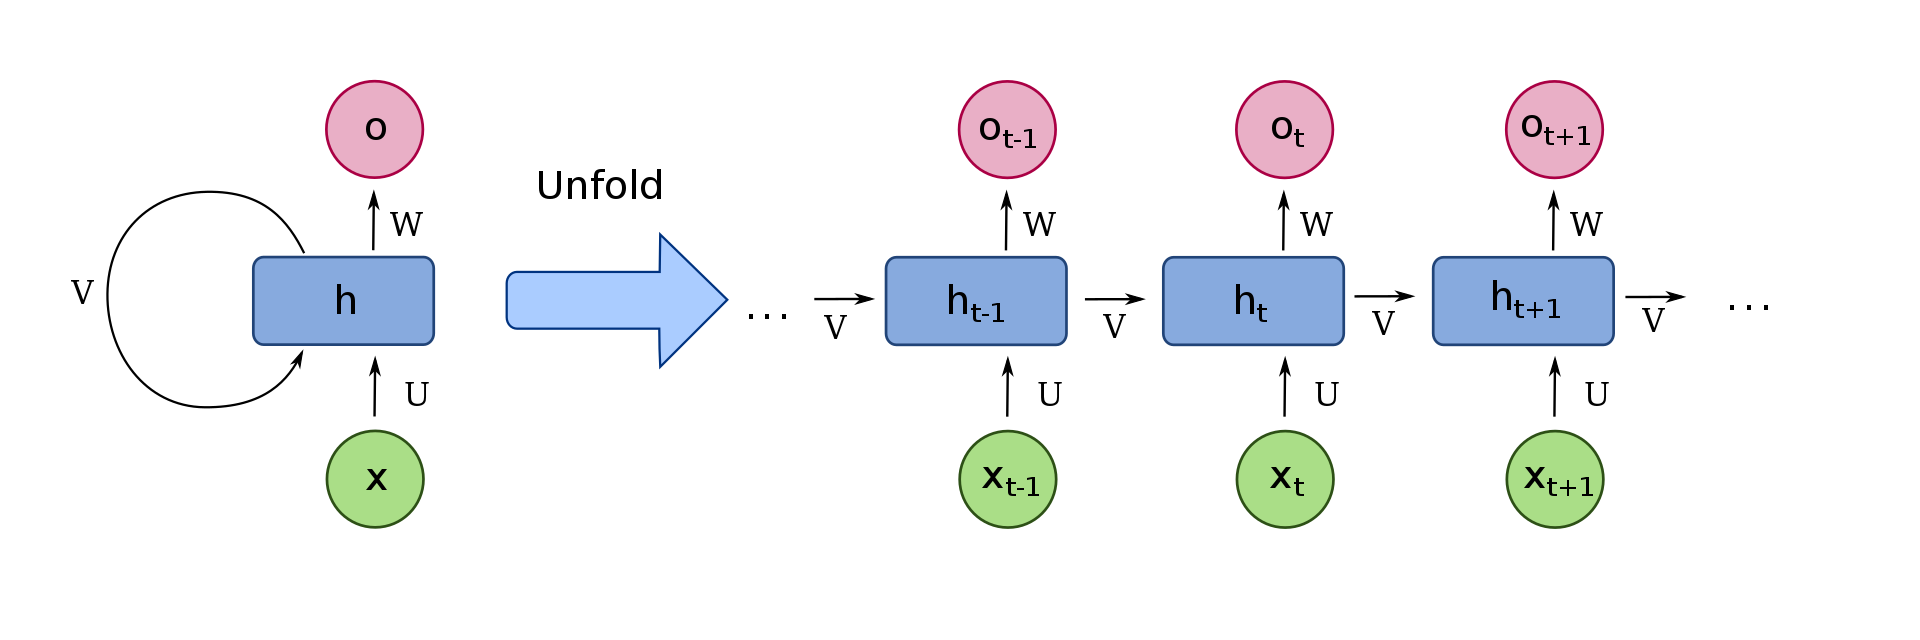
\includegraphics[width=\columnwidth]{figures/rnn.png}%
\caption{Schéma d'un réseau récurrent. A droite la version compression, à gauche la version dépliée sur chaque entrée (source:~\cite{lecun2015deep})}%
\label{fig:rnn}%
\end{figure}

Une limitation significative des modèles RNN simples est la disparition du gradient (\textit{vanishing gradient}~\cite{hochreiter1998vanishing}).
La capacité à rétro-propager un signal d'erreur à travers le temps devient de plus en plus difficile.
De la même manière qu'avec les réseaux très profonds type ResNet, le gradient devient trop faible à mesure que le réseau devient profond.
Les blocs LSTM (Long Short-Term Memory) permettent un apprentissage plus profond grâce à des mécanismes non linéaire pour transmettre l'état caché, qui est alors soit propagé sans modification, être mise à jour ou réinitialisé grâce à des portes de connection~\cite{hochreiter1997long}.

Les LSTM, et leur dérivés comme les GRU~\cite{cho2014learning}, ont permis des avancées dans la reconnaissance d'action et d'évènement dans les vidéos.
Couplés avec un CNN pour réaliser l'extraction de caractéristique spatiale, les LSTM font office de fusion d'information temporelle.
On voit sur la figure~\ref{fig:cnnlstm} l'utilisation typique d'un CNN et d'un LSTM pour classifier un segment de vidéo.
Bien que ces approches présentent généralement les meilleures performances~\cite{donahue2015long, yue2015beyond, srivastava2015unsupervised, yao2015video}, elles présentent le problème d'être coûteuse en terme de calcul, et de plus, nécessite que chaque trame de la vidéo soit passée dans le réseau de neurones, ce qui augmente grandement le nombre de calcul à effectuer.
Dans le cadre d'une application mobile, pour limiter le nombre de paramètres, l'occupation mémoire et le temps de calcul, nous nous basons dans le chapitre~\ref{chap:gestes}, sur des méthodes à bases de CNN uniquement.

\begin{figure}[ht!]
\centering
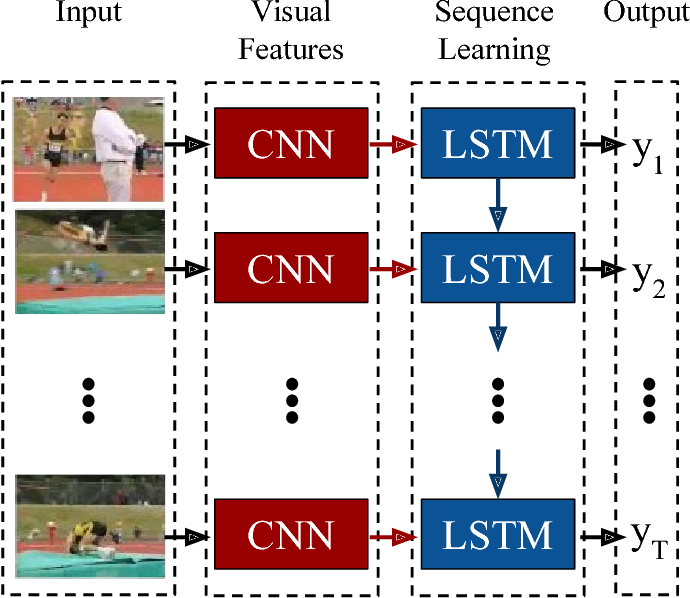
\includegraphics[width=\columnwidth]{figures/cnnlstm.png}%
\caption{Réseaux récurrents pour la detection d'action dans les vidéos à base de CNN et de LSTM (source~\cite{donahue2015long})}%
\label{fig:cnnlstm}%
\end{figure}


\section{Conclusion}

Nous avons présenté dans ce chapitre les méthodes existantes pour la recherche d’instances.
Dans les chapitres~\ref{chap:similarite} et~\ref{chap:regions}, nous présentons nos propositions pour adapter ces méthodes à nos problématiques, et améliorer les résultats dans le cas de la recherche d’instances en mobilité. 

La proposition de Gordo et al.~\cite{gordo2016deep}, présente les meilleurs résultats pour la recherche d’instances.
Cependant elle requiert l’utilisation de régions annotées sur les images, ce dont nous ne disposons pas. 
Dans le chapitre suivant, nous adaptons les réseaux siamois à trois branche, avec un modèle proche de celui de FaceNet, avec une sélection de triplets adaptée à nos collection. 
Les réseaux à proposition de régions présentent les meilleurs résultats et donc, dans le chapitre~\ref{chap:regions}, nous étudions les possibilité de régions sans annotation dans la collection.

Pour la détection de gestes, dans le chapitre~\ref{chap:gestes}, nous n’utilisons pas les réseaux récursifs, par un soucis de temps de calcul et d’occupation mémoire sur processeur mobile.
Nous nous intéressons à la fusion d’information temporelle à l’intérieur du réseau à la manière de Karparthy et al.~\cite{karpathy2014large}, avec comme objectif de réduire le nombre de paramètres.

